\PassOptionsToPackage{svgnames}{xcolor}
\documentclass[12pt]{article}



\usepackage[margin=1in]{geometry}  
\usepackage{graphicx}             
\usepackage{amsmath}              
\usepackage{amsfonts}              
\usepackage{framed}               
\usepackage{amssymb}
\usepackage{array}
\usepackage{amsthm}
\usepackage{multirow}
\usepackage[nottoc]{tocbibind}
\usepackage{bm}
\usepackage{enumitem}
\usepackage{tikz}
\newcolumntype{C}[1]{>{\centering\let\newline\\\arraybackslash\hspace{0pt}}m{#1}}


  \newcommand\norm[1]{\left\lVert#1\right\rVert}
\setlength{\parindent}{0cm}
\setlength{\parskip}{0em}
\newcommand{\Lim}[1]{\raisebox{0.5ex}{\scalebox{0.8}{$\displaystyle \lim_{#1}\;$}}}
\newtheorem{definition}{Definition}[section]
\newtheorem{theorem}{Theorem}[section]
\newtheorem{notation}{Notation}[section]
\theoremstyle{definition}
\DeclareMathOperator{\arcsec}{arcsec}
\DeclareMathOperator{\arccot}{arccot}
\DeclareMathOperator{\arccsc}{arccsc}
\DeclareMathOperator{\spn}{Span}
\setcounter{tocdepth}{1}
\begin{document}
\tikzstyle{block} = [draw, rectangle, minimum height=2em, minimum width=3em]
\tikzstyle{virtual} = [ draw, rectangle, minimum height=2em, minimum width=3em]
\title{Revision notes - CS2100}
\author{Ma Hongqiang}
\maketitle
\tableofcontents

\clearpage
%\twocolumn
\section{Introduction}
\begin{definition}[Computer]
\hfill\\\normalfont
A computer is a device capable of solving problems according to designed programs. It simply augments our power of storage and speed of calculation. 
\begin{figure}[h]
\centering
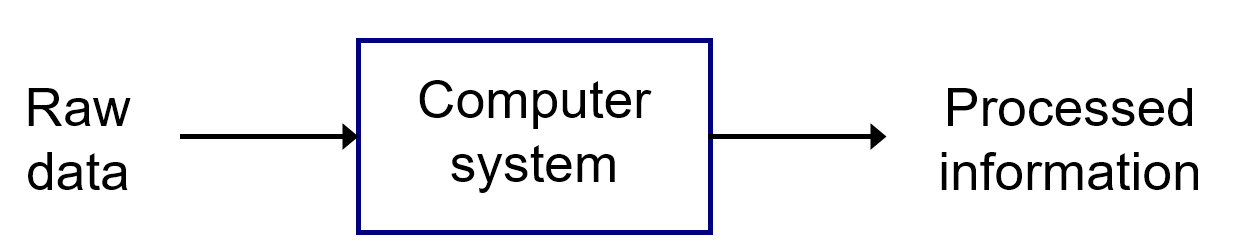
\includegraphics[width = 0.5\textwidth]{1_1.png}
\caption{Computers as information processors.}
\end{figure}
\end{definition}
\begin{definition}[Hardware Stack]
\hfill\\\normalfont The hardware stack with the most basic on the top goes like: 
\begin{itemize}
  \item Transistor
  \item Logic Gate
  \item Circuits
  \item Memory
  \item Processor
\end{itemize}
\end{definition}
\begin{definition}[Transistor]
\hfill\\\normalfont A \textbf{transistor} is
\begin{itemize}
  \item a \textit{solid state switch}. The input switches on or off the output.
  \item It is also an \textit{amplifier}. The output signal is much stronger than the input so that things can be connected up.
\end{itemize}
\end{definition}
\begin{definition}[Boolean logic gates]t
\hfill\\\normalfont To compute, \textbf{Boolean logic gates} is built by transistors to compute Boolean logic functions.
\end{definition}
The basic Boolean logic gates include:
\begin{itemize}
  \item NOT
  \item OR, AND
  \item NAND, NOR
\end{itemize}
\clearpage
\begin{theorem}[Behaviour of nMOS and pMOS transistor]
\hfill\\\normalfont
\begin{figure}[h]
\centering
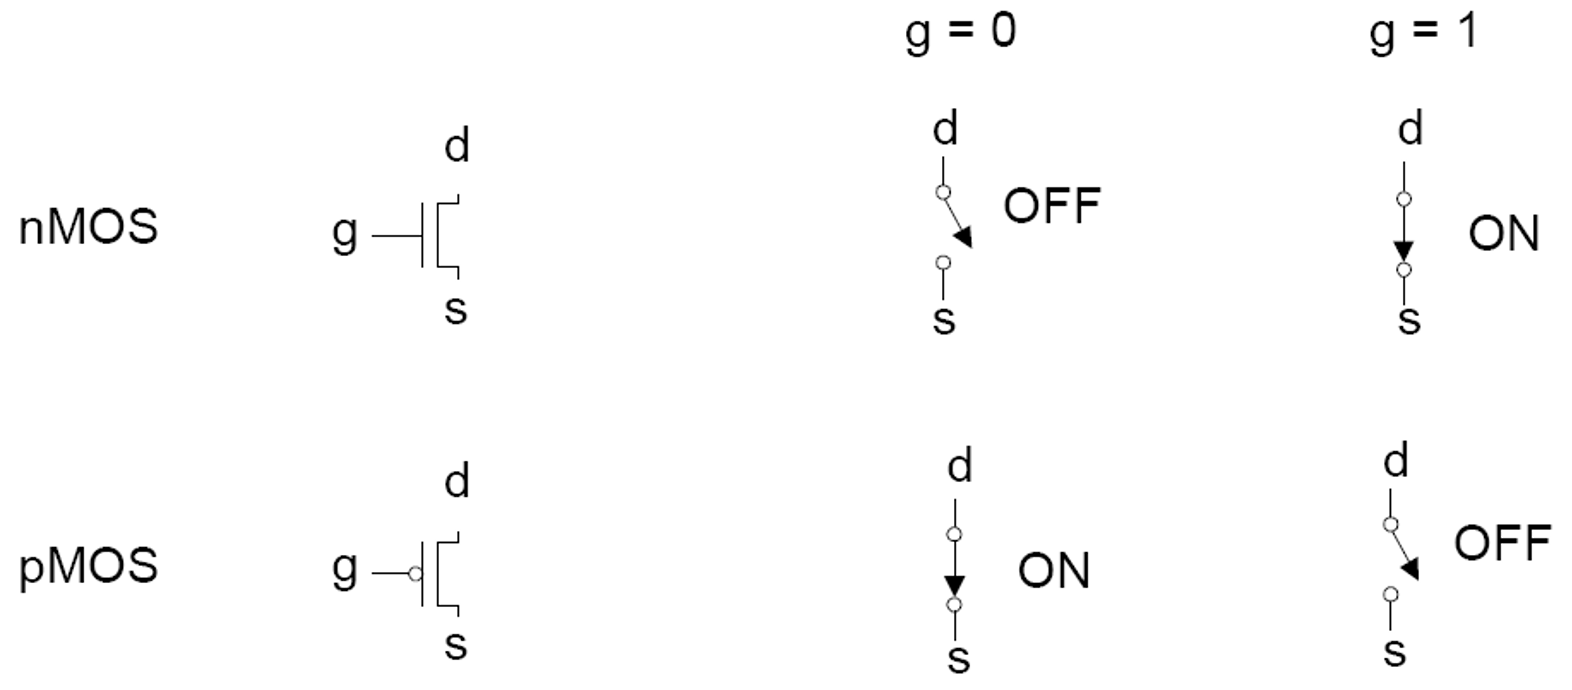
\includegraphics[width = 0.7\textwidth]{1_2.png}
\end{figure}
\end{theorem}
Examples of logic gates constructed by nMOS and pMOS include:
\begin{figure}[h]
\centering
\begin{minipage}{0.45\textwidth}
  \centering
  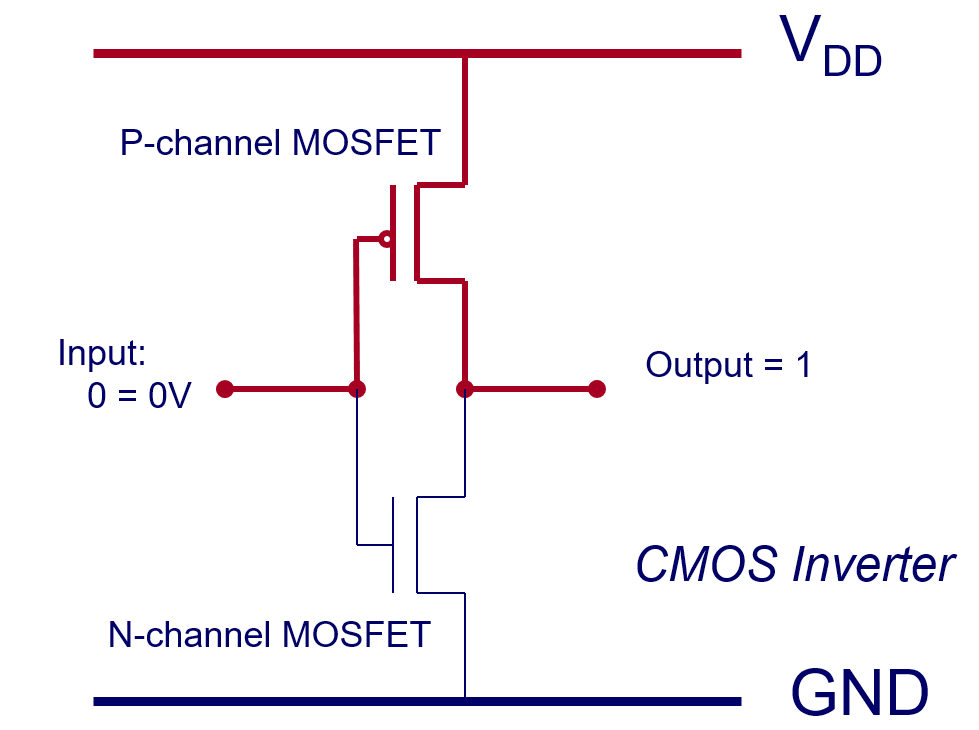
\includegraphics[width = \textwidth]{1_3.png}
  \caption{CMOS NOT Gate}
\end{minipage}
\hfill
\begin{minipage}{0.45\textwidth}
  \centering
  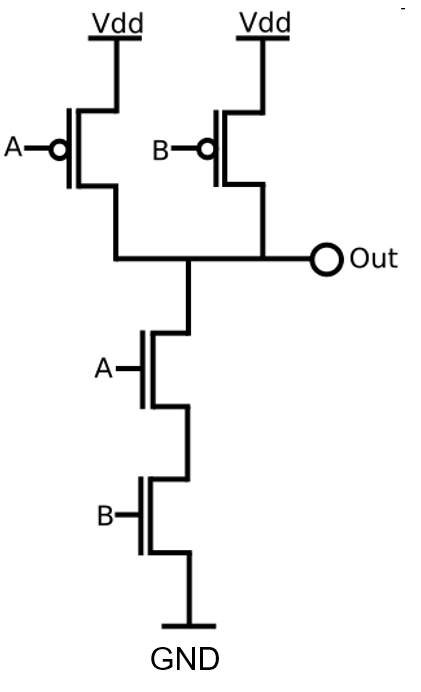
\includegraphics[width = 0.6\textwidth]{1_4.png}
  \caption{CMOS NAND Gate}
\end{minipage}
\end{figure}
\clearpage
\section{Number Systems}
\subsection{Information Representation}
\begin{definition}[Bit]
\hfill\\\normalfont \textbf{Bit} is the short form of \textit{bi}nary digi\textit{t}.
\begin{itemize}
  \item 0 and 1
  \item Represent \texttt{false} and \texttt{true} in logic
  \item Represent the \textit{low} and \textit{high} states in electronic devices
\end{itemize}
\end{definition}
Other units include
\begin{itemize}
  \item Byte: 8 bits
  \item Nibble: 4 bits
  \item Word: Multiple of byte
\end{itemize}
Obviously, $N$ bits can represent up to $2^N$ values.\\
Conversely, to represent $M$ values, $\log_2 M$ bits are required.
\begin{definition}[Weighted-positional Number System]
\hfill\\\normalfont A \textbf{weighted-positional number system} is one whose
\begin{itemize}
  \item \textbf{Base} or \textbf{radix} is $N$.
  \item position is important, as the value of each symbol/digit is dependent on its \textbf{type} and \textbf{position} in the number.
  \item In general, 
  \[
(a_na_{n-1}\cdot a_1a_0.b_1b_2\cdot)_N = \sum_{k= 0}^n a_kN^k + \sum_{k=1}^\infty b_kN^{-k}
  \]
\end{itemize}
\end{definition}
For example, in the decimal number system, 
\[
(593.68)_{10} = 5\times 10^2 + 9\times 10^1 +3\times 10^0+6\times 10^{-1}+8\times 10^{-2}
\]
The method of conversion between bases can be found in \texttt{MA2213 Revision Note}.\\
In special cases, binary can be converted to octal and hexadecimal by partitioning the number in groups of 3 and 4 respectively.
\subsection{Signed Binary Number}
Any real number can be converted to a signed binary number. A \textbf{signed binary number} is defined by its
\begin{itemize}
\item \textbf{sign}
\item \textbf{absolute value}
\end{itemize}
In general, a signed binary number can be represented as \[
\pm a_{n-1}a_{n-2}\cdots a_0.b_1b_2\cdots\] where $a_i, b_j = 0\text{ or }1$ for $i = [0..n]$,\;\;\;$j=\mathbb{Z}^+$.   
\begin{definition}[String Representation of Signed Binary Number]
\hfill\\\normalfont A \textbf{string representation} of signed binary numbers is a \textbf{bijection} from \textbf{signed binary numbers} to \textbf{strings of bits}.\\
Specifically for binary integers with sign $s$ and absolute value $v$, define the bijective function $f$:
\begin{align*}
f:(\text{sign},\text{absolute value})&\to \text{binary }\texttt{String}\\
(s,v)&\mapsto \texttt{str}
\end{align*}
where \texttt{str} is the string representation $f$ of that particular signed binary number defined by $s$ and $v$.
\end{definition}
\begin{definition}[Negation of String Representation]
\hfill\\\normalfont 
Negation is a unitary function $-$:
\begin{align*}
-:\text{binary }\texttt{String}&\to \text{binary }\texttt{String}\\
\texttt{str}&\mapsto -\texttt{str}
\end{align*}
where $
-\texttt{str}:=f(-s,v)
$
\end{definition}
There are three common string representations of signed binary number, namely
\begin{itemize}
  \item Sign-and-Magnitude $f_\text{sm}$
  \item 1s complement $f_{1\text{s}}$
  \item 2s complement $f_{2\text{s}}$
\end{itemize}
In the rest of this subsection, the length of string \texttt{str} is fixed to $n$, and $\texttt{str} = a_{n-1}a_{n-2}\cdots a_0$.
\subsubsection{Sign-and-Magnitude Representation $f_\text{sm}$}
\begin{definition}[$f_\text{sm}$]
\hfill\\\normalfont
  In \textbf{sign-and-magnitude} representation, sign $s$ is represented by a \textbf{sign bit} in the leftmost position of string \texttt{str}, i,e, $a_{n-1}$.
\begin{itemize}
  \item 0 for $+$
  \item 1 for $-$
\end{itemize}
The absolute value $v$ will occupy the rest $n-1$ bits of \texttt{str}: $a_{n-2}a_{n-3}\cdots a_0:=v$.\\
For a $n$ bit sign-and-magnitude representation, the domain of $f_\text{sm}$ is $[-2^{n-1}+1,2^{n-1}-1]\cap\mathbb{Z}$.
\end{definition}
Clearly, say, for 8-bit sign-and-magnitude representation,
\begin{itemize}
\item \textbf{Largest value}: $01111111_{\text{sm}}=+127_{10}$
\item \textbf{Smallest value}: $11111111_{\text{sm}}=-127_{10}$
\item \textbf{Zeros}: $00000000_{\text{sm}}= +0_{10}$ and $10000000_{\text{sm}}=-0_{10}$
\item \textbf{Range}: $-127_{10}$ to $+127_{10}$
\end{itemize}
\begin{theorem}[Negation of $str$ in sign-and-magnitude representation]
\hfill\\\normalfont To \textbf{negate} a \texttt{str} in sign-and-magnitude interpretation, \textbf{invert the sign bit}\footnote{Inversion of bit $b$ is denoted by $\overline{b}$}.
Suppose $\texttt{str} = a_{n-1}a_{n-2}\cdots a_0$, then
\[
-\texttt{str} = \overline{a_{n-1}}a_{n-2}\cdots a_0
\]
\end{theorem}
\begin{theorem}[$f^{-1}_\text{sm}$]
\hfill\\\normalfont $f^{-1}(\texttt{str})$ is defined\footnote{$f^{-1}$ is well defined as $f$ is a bijection} as follows:
\begin{align*}
f^{-1}_\text{sm}(\texttt{str})&=f^{-1}(a_{n-1}a_{n-2}\cdots a_0)\\
:&=(-1)^{a_{n-1}}\times\sum_{i=0}^{n-2}(a_i\times 2^i)
\end{align*}
\end{theorem}
\subsubsection{1s Complement}
\begin{definition}[$f_\text{1s}$ for non-negative binary numbers]
\hfill\\\normalfont
Suppose a \textbf{nonnegative} number is defined by $(+,v)$. In \textbf{1s complement} representation \texttt{str}, 
\begin{itemize}
\item the positive sign defines $a_{n-1}:=0$;
\item the absolute value $v$ will occupy the rest $n-1$ bits of \texttt{str}: $a_{n-2}a_{n-3}\cdots a_0:=v$.
\end{itemize}
\end{definition}
\begin{definition}[Negation]
\hfill\\\normalfont Negation of 1s complement representation is defined as:
\begin{align*}
-:\text{binary }\texttt{String}&\to \text{binary }\texttt{String}\\
\texttt{str}=a_{n-1}a_{n-2}\cdots a_0&\mapsto \overline{a_{n-1}a_{n-2}\cdots a_0}:=-\texttt{str}
\end{align*}
Essentially, to negate a \texttt{String} of 1s complement, \textbf{invert all the bits}.
\end{definition}
\begin{definition}[$f_\text{1s}$ for non-positive binary numbers]
\hfill\\\normalfont
The 1s complement representation of a \textbf{non-positive binary number} defined by $(-,v)$ is defined by \textbf{negation} of $f_\text{1s}((+,v))$.\\
Essentially,
\[
\texttt{str}=1\overline{a_{n-2}a_{n-3}\cdots a_0}
\]
Together with the previous definition, for a $n$ bit 1s complement representation, the domain of $f_\text{1s}$ is $[-2^{n-1}+1,2^{n-1}-1]\cap\mathbb{Z}$.
\end{definition}
Clearly, say, for 8-bit 1s complement representation,
\begin{itemize}
  \item \textbf{Largest value}: $01111111_{\text{1s}} = +127_{10}$
  \item \textbf{Smallest value}: $10000000_{\text{1s}}=-127_{10}$
  \item \textbf{Zeros}: $00000000_\text{1s}=+0_{10}$ and $11111111_\text{1s} = -0_{10}$
  \item \textbf{Range}: $-127_{10}$ to $+127_{10}$.
\end{itemize}
\begin{theorem}[Sign Bit of 1s Complement]
\hfill\\\normalfont The leftmost position of string \texttt{str}, i,e, $a_{n-1}$, still represents the sign:
\begin{itemize}
  \item 0 for $+$
  \item 1 for $-$
\end{itemize}
\end{theorem}
\begin{theorem}[$f^{-1}_\text{1s}$]
\hfill\\\normalfont $f^{-1}(\texttt{str})$ is defined as follows:
\begin{align*}
f^{-1}_{\text{1s}}(\texttt{str})&=f^{-1}(a_{n-1}a_{n-2}\cdots a_0)\\
:&=((-2^{n-1}+1)\times a_{n-1})+\sum_{i=0}^{n-2}a_i\times 2^i
\end{align*}
\end{theorem}
\subsubsection{2s Complement}
\begin{definition}[$f_\text{2s}$ for non-negative binary numbers]
\hfill\\\normalfont
Suppose a \textbf{nonnegative} number is defined by $(+,v)$. In \textbf{2s complement} representation \texttt{str}, 
\begin{itemize}
\item the positive sign defines $a_{n-1}:=0$;
\item the absolute value $v$ will occupy the rest $n-1$ bits of \texttt{str}: $a_{n-2}a_{n-3}\cdots a_0:=v$.
\end{itemize}
\end{definition}
\begin{definition}[Negation]
\hfill\\\normalfont Negation of 2s complement representation is defined as:
\begin{align*}
-:\text{binary }\texttt{String}&\to \text{binary }\texttt{String}\\
\texttt{str}=a_{n-1}a_{n-2}\cdots a_0&\mapsto \texttt{(String)}(\texttt{(binary number)}\overline{a_{n-1}a_{n-2}\cdots a_0}+1):=-\texttt{str}
\end{align*}
Essentially, negation of a \texttt{String} of 2s complement equals to the sum of this \texttt{String} with all bits flipped and 1.
\end{definition}
\begin{definition}[$f_\text{2s}$ for negative binary numbers]
\hfill\\\normalfont
The 2s complement representation of a \textbf{negative binary number} defined by $(-,v)$ is defined by \textbf{negation} of $f_\text{2s}((+,v))$.\\
Essentially,
\[
\texttt{str}= \overline{a_{n-1}a_{n-2}\cdots a_0}+1
\]
Together with the previous definition, for a $n$ bit 2s complement representation, the domain of $f_\text{2s}$ is $[-2^{n-1},2^{n-1}-1]\cap\mathbb{Z}$.
\end{definition}
Clearly, say, for 8-bit 2s complement representation,
\begin{itemize}
  \item \textbf{Largest value}: $01111111_{\text{2s}} = +127_{10}$
  \item \textbf{Smallest value}: $10000000_{\text{2s}}=-128_{10}$
  \item \textbf{Zeros}: $00000000_\text{2s}=+0_{10}$
  \item \textbf{Range}: $-128_{10}$ to $+127_{10}$.
\end{itemize}
\begin{theorem}[Sign Bit of 2s Complement]
\hfill\\\normalfont The leftmost position of string \texttt{str}, i,e, $a_{n-1}$, still represents the sign:
\begin{itemize}
  \item 0 for $+$
  \item 1 for $-$
\end{itemize}
\end{theorem}
\begin{theorem}[$f^{-1}_\text{2s}$]
\hfill\\\normalfont $f^{-1}_\text{2s}(\texttt{str})$ is defined as follows:
\begin{align*}
f^{-1}_\text{2s}(\texttt{str})&=f^{-1}_\text{2s}(a_{n-1}a_{n-2}\cdots a_0)\\
:&=(-2^{n-1}\times a_{n-1})+\sum_{i=0}^{n-2}a_i\times 2^i
\end{align*}
\end{theorem}
\subsection{Generalising complement}
\begin{definition}[$(r-1)$'s complement]
\hfill\\\normalfont Let $a_{n-1}a_{n-2}\cdots a_{0}$ be string representation of a number in radix $r$. The (r-1)\textbf{'s complement} is the string $\overline{a_{n-1}a_{n-2}\cdots a_{0}}$ where $\overline{a_{i}}=r-1-a_{i}$.
\end{definition}
The $r$\textbf{'s complement} is just the $(r-1)$'s complement with 1 added to the least significant bit.
\begin{theorem}[Complement on Fractions]
\hfill\\\normalfont We can extend the operations of complement on fractions.
\end{theorem}
\begin{theorem}[2s Complement Addition/Subtraction]
\hfill\\\normalfont Algorithm for \textbf{addition}, $A_\text{2s}+B_\text{2s}$:
\begin{itemize}
  \item Perform binary addition on the two \texttt{(binary number) String}.
  \item Ignore the carry out of the most significant bit(MSB).
  \item Check for overflow. Overflow occurs if
  \begin{enumerate}
    \item the 'carry in' and 'carry out' of the MSB are different, or
    \item result is of opposite sign of $A_\text{2s}$ and $B_\text{2s}$.
  \end{enumerate}
\end{itemize}
Algorithm for \textbf{subtraction} $A_\text{2s}-B_\text{2s}$: $A_\text{2s}-B_\text{2s}=A_\text{2s}+(-B)_\text{2s}$.
\end{theorem}
\begin{theorem}[1s Complement Addition/Subtraction]
\hfill\\\normalfont Algorithm for \textbf{addition}, $A_\text{1s}+B_\text{1s}$:
\begin{itemize}
  \item Perform binary addition on the two \texttt{(binary number) String}.
  \item If there is a carry out of the MSB, add 1 to the result.
  \item Check for overflow. Overflow occurs if
  \begin{enumerate}
      \item result is of opposite sign of $A_\text{1s}$ and $B_\text{1s}$.
  \end{enumerate}
\end{itemize}
Algorithm for \textbf{subtraction} $A_\text{1s}-B_\text{1s}$: $A_\text{1s}-B_\text{1s}=A_\text{1s}+(-B)_\text{1s}$.
\end{theorem}
\subsection{Excess-$k$ Representation}
\begin{definition}[$f_{\text{excess}-k}$]
\hfill\\\normalfont
Suppose a number $N$ is defined by $(s,v)$. Clearly, this number $N$ equals $\text{sgn}(s)\times v$.Its \textbf{excess}-$k$ representation($k>0$) \texttt{str} is defined as
\[
\texttt{str}=f_{\text{excess}-k}((s,v)):=f_\text{sm}(N+k)
\] 
\end{definition}
For a $n$ bit excess-$k$ complement representation, the domain is $[-k, 2^n-k-1]\cap \mathbb{Z}$.\\
Note: $\texttt{k}_{\text{excess}-k}=k_2$ numerically.
\begin{definition}[Negation]
\hfill\\\normalfont Negation of excess-$k$ representation of is calculated as:
\[
-\texttt{str}:=\texttt{String}(2\times k-\texttt{(binary number)} \texttt{str})
\]
\end{definition}
Domain of the above negation operation is $[-\min\{2^n-k-1,k\},\min\{2^n-k-1,k\}]$ if $k<2^n$ and $\varnothing$ otherwise.\\
There is no \textbf{sign bit} for excess-$k$ representation.
\begin{definition}[$f_{\text{excess}-k}^{-1}$]
\hfill\\\normalfont $f_{\text{excess}-k}^{-1}$ is defined as follows:
\[
f_{\text{excess}-k}^{-1}(\texttt{str})=\texttt{(binary number)} \texttt{str}-k
\]
\end{definition}
\subsection{Floating Point Numbers}
\begin{definition}[Fixed Point Numbers]
\hfill\\\normalfont In fixed point representation, the binary point is assumed to be at fixed location.\\In general, the binary point may be assumed to be at any pre-fixed location.
\end{definition}
Fixed point numbers have limited range. Floating point numbers allow us to represent very large or very small numbers.
\begin{definition}[Floating Point Numbers]
\hfill\\\normalfont \textbf{Floating point numbers} consists of 3 parts: \textbf{sign}, \textbf{mantissa} and \textbf{exponent}.
\end{definition}
\begin{itemize}
  \item The base (radix) is assumed to be $2$.
  \item Sign bit: 0 for positive, 1 for negative.
  \item Mantissa is usually in \textbf{normalised form}.
\end{itemize}
Clearly, the trade-off of floating point numbers is
\begin{itemize}
  \item More bits in mantissa $\rightarrow$ better precision
  \item More bits in exponent $\rightarrow$ larger range of values
\end{itemize}
\begin{definition}[IEEE Standard 754]
\hfill\\\normalfont IEEE Standard 754 has the following properties:
\begin{itemize}
  \item Two types of formats
  \begin{itemize}
    \item \textbf{Normalised} numbers
    \item \textbf{Denormalised} numbers
  \end{itemize}
  \item Special values
  \begin{itemize}
    \item Negative zero
    \item Infinities
    \item Not-a-Number(NaN)
  \end{itemize}
  \item Distribution of bits in mantissa and exponent: See table below
\end{itemize}
\begin{table}[h]
\centering
\begin{tabular}{|l|r|r|}
\hline
Parameter&Single&Double\\\hline
No. of fraction bits  &23&52\\\hline
Maximum exponent      &+127&+1023\\\hline
Minimum exponent      &-126&-1022\\\hline
Exponent bias         &+127&+1023\\\hline
Exponent width in bits&8&11\\\hline
Format width in bits  &32&64\\\hline
\end{tabular}
\end{table}
\end{definition}
\clearpage
The IEEE Standard 754 admits the following format:
\begin{figure}[h]
\centering
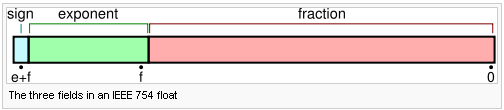
\includegraphics[width = 0.8\textwidth]{2_1.png}
\end{figure}
\begin{definition}[Normalised Number]
\hfill\\\normalfont A \textbf{normalised number},$v$, represented in IEEE 754 is
\[
v = (-1)^\text{sign}\times 1.\text{fraction}\times 2^{\text{exponent}-bias}
\]
Note: for normalised numbers, the integer part of the 8 bit fraction part is 1.
\begin{itemize}
  \item Sign bit is 1 bit, followed by exponent and lastly mantissa
  \item Exponent must NOT be $0$. It must be in $[1,2^e-2]$, where $e$ is the number of exponent bits.\\ All zero $0$ or all one $2^e-1$ exponents are reserved for special values and are not used for normalised numbers
  \item Suppose the exponent bias is $b$, then the exponent is in excess-$b$ representation of the true power.
  \item A normalised fraction part is in the interval $[1,2)$.
\end{itemize}
\end{definition}
\begin{definition}[Denormalised numbers]
\hfill\\\normalfont \textbf{Denormalised numbers} are to represent really small (positive or negative) numbers as following:
\[
v=(-1)^\text{sign}\times 0.\text{fraction}\times 2^{-\text{bias}s+1} 
\]
To identify a number as \textbf{denormalised}, exponent must be 0 and mantissa must be non-zero.\\
The system will interpret the exponent to be $1-\text{bias}$ instead of $0_\text{excess-bias}$.
\end{definition}
\begin{definition}[Special values]
\hfill\\\normalfont
\begin{itemize}
  \item \makebox[1.5cm]{$0$:\hfill}\makebox[4cm]{exponent = 0\hfill}\makebox[3cm]{fraction = 0\hfill}
  \item \makebox[1.5cm]{$+\infty$:\hfill}\makebox[4cm]{exponent = $2^e-1$\hfill}\makebox[3cm]{fraction = $0$\hfill}
  \item \makebox[1.5cm]{$-\infty$:\hfill}\makebox[4cm]{exponent = $2^e-1$\hfill}\makebox[3cm]{fraction = 0\hfill}
  \item \makebox[1.5cm]{NaN:\hfill}\makebox[4cm]{exponent = $2^e-1$\hfill}\makebox[3cm]{fraction $\neq$ 0\hfill} 
\end{itemize}
\end{definition}
\begin{table}[h]
\centering
\begin{tabular}{|c|c|c|c|}
\hline
Type&Sign&Exponent&Fraction\\\hline
$+\infty$&0&$\underbrace{11\cdots1}_{e}$& $\underbrace{0\cdots0}_{f}$\\\hline
$-\infty$&1&$\underbrace{11\cdots1}_{e}$& $\underbrace{0\cdots0}_{f}$\\\hline
NaN&&$\underbrace{11\cdots1}_{e}$& non zero\\\hline
$0$&    &$\underbrace{00\cdots0}_{e}$       &$\underbrace{00\cdots0}_{f}$       \\\hline
Denormalised Numbers&&$\underbrace{0\cdots0}_{e}$& non zero\\\hline
Normalised Numbers&&$[\underbrace{00\cdots 0}_{e-1}1,\underbrace{11\cdots1}_{e-1}0]$&$[\underbrace{00\cdots 0}_{f},\underbrace{11\cdots1}_{f}]$\\\hline
\end{tabular}
\end{table}
\begin{definition}[Comparison Rules]
\hfill\\\normalfont 
\begin{itemize}
  \item Negative and positive zero compare \textit{equal}
  \item Every NaN compares \textit{unequal} to every value, including itself
  \item All values except NaN are strictly smaller than $+\infty$ and strictly larger than $-\infty$.
\end{itemize}
\end{definition}
\begin{definition}[Overflow, Underflow]
In floating point representation, greater than the largest representable positive number or smaller than the smallest representable negative number results in \textbf{overflow}; greater than the largest representable negative number and smaller than the smallest representable positive number results in \textbf{underflow}.
\end{definition}
\begin{definition}[Rounding]
\hfill\\\normalfont \textbf{Rounding} is defined as selecting a representable number as the result, from the two closest representable numbers.
\end{definition}
Rounding destroys associativity of all operations on floating point numbers.\\
\begin{definition}[Guard Bit, Round Bit, Sticky Bit]\hfill\\\normalfont
To enable rounding, IEEE 754 specifies that all arithmetic must be performed with 3 extra bits at the end of the last fraction bit, from the order of the most significant bit to the least:
\begin{itemize}
  \item Guard bit
  \item Round bit
  \item Sticky bit, which equals to 1 if any bits to the right of it is 1
\end{itemize}
\end{definition}
\begin{figure}[h]
\centering
  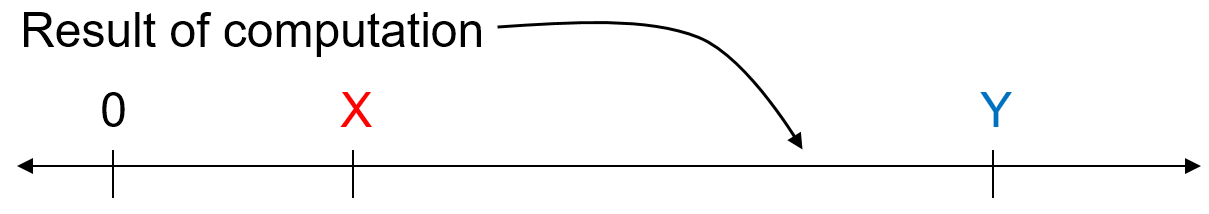
\includegraphics[width = 0.7\textwidth]{2_2.png}
\end{figure}
\begin{theorem}[Rounding Modes]\hfill\\\normalfont
There are four rounding modes:
\begin{itemize}
  \item Round to nearest (default)
  \begin{verbatim}
if (GUARD == 1) {
  if ((ROUND == 1) or (STICKY == 1)) {
    return Y as the mantissa answer
  } else { // Must be (ROUND == 0) and (STICKY == 0)
    // Invoke IEEE tie breaker
    if (LSB, i.e., bit 23 is 1) {
      return Y as the mantissa answer
    } else {
      return X as the mantissa answer
    }
  }
} else {
    return X as the mantissa answer
}
\end{verbatim}
  \item Round towards $0$
  \begin{verbatim}
Always report X as the mantissa answer.
(if less than 0, then this becomes –X)
\end{verbatim}
  \item Round towards $+\infty$
  \begin{verbatim}
if (result > 0) {
   report Y as the mantissa answer.
} else {
   report X as the mantissa answer.
}
\end{verbatim}
  \item Round towards $-\infty$
\begin{verbatim}
if (result < 0) {
   report Y as the mantissa answer.
} else {
   report X as the mantissa answer.
}
\end{verbatim}
\end{itemize}
\end{theorem}
\begin{definition}[Error]
\hfill\\\normalfont Rounding yields a representable floating point number $x^\prime$ that is an approximation of the real number $x$.\\
Define absolute error = $|x^\prime -x|$.\\
Define relative error = $\frac{|x^\prime -x|}{x}$ (assuming $x\neq 0$)
\end{definition}
\begin{definition}[Machine Epsilon $\varepsilon$]
\hfill\\\normalfont Informally, \textbf{machine epsilon} $\varepsilon$ is defined as 1\textit{ added to the LSB}.
\end{definition}
\begin{definition}[Unit in the Last Place(ulp)]
\hfill\\\normalfont Given an IEEE floating point number $x$, say with an exponent $E$. The \textbf{unit in the last place} of $x$ is defined as
\[
\text{ulp}(x)=\varepsilon\times 2^E
\]
\end{definition}
\textbf{Round to nearest} results in an absolute error that is less than $\frac{1}{2}\text{ulp}(x)$.
\begin{theorem}[Floating Point Addition]
\hfill\\\normalfont Given two decimal numbers in floating point notation:
\begin{itemize}
  \item $X=0.a_1a_2\cdots a_n\times 2^p$
  \item $Y=0.b_1b_2\cdots b_n\times 2^q$
\end{itemize}
To perform $X+Y$,
\begin{enumerate}
\item align the decimal point by shifts such that two exponents are the same.
\item If $p>q$, then we need to adjust $Y$ such that $Y^\prime = 0.\underbrace{00\cdots 0}_{p-q}b_1b_2\cdots b_n\times 2^p$.\\ This is called \textbf{denormalisation shift}.
\item Addition is performed on fraction part of $X$ and $Y$.
\item Normalise the result
\item Round the result
\end{enumerate}
\end{theorem}
\clearpage
\section{Boolean Algebra}
\begin{definition}[Digital Circuit]
\hfill\\\normalfont \textbf{Digital circuit} is circuit with two voltage levels, known as
\begin{itemize}
  \item High, true, 1, asserted
  \item Low, false, 0, deasserted
\end{itemize}
\end{definition}
Advantages of digital circuits over analog circuits include:
\begin{itemize}
  \item More reliable (simpler circuits, less noise-prone)
  \item Specified accuracy (determinable)
  \item Abstraction can be applied using simple mathematical model -- Boolean Algebra
  \item Ease design, analysis and simplification of digital circuit -- Digital Logic Design
\end{itemize}
\begin{definition}[Type of Logic Blocks]
\hfill\\\normalfont There are two types of logic blocks, known as
\begin{enumerate}
  \item \textbf{Combinatorial}: \textit{no} memory, output depends \textit{solely} on the input
  \begin{itemize}
    \item Gates
    \item Decoders, multiplexers
    \item Adders, multipliers
  \end{itemize}
  \item \textbf{Sequential}: \textit{with} memory, output depends on \textit{both} input and \textit{current states}
  \begin{itemize}
    \item Counters, registers
    \item Memories
  \end{itemize}
\end{enumerate}
\end{definition}
\subsection{Boolean Algebra}
Boolean algebra involves \textbf{boolean values} and \textbf{connectives}.
\begin{definition}[Boolean Values]
\hfill\\\normalfont There are \textit{two} \textbf{boolean values} in boolean algebra:
\begin{itemize}
  \item True (1)
  \item False (0)
\end{itemize}
\end{definition}
\begin{definition}[Connectives]
\hfill\\\normalfont There are \textit{three} \textbf{connectives} in boolean algebra, which maps given input boolean value(s) to a single output boolean value.\\
\textbf{Truth tables} defines a connective by providing a listing of every possible combination of inputs and its corresponding outputs.\\
\textbf{Reminder}: Inputs must list in \textit{ascending} \textbf{binary sequence}.\\
The three connectives are:\clearpage
\begin{itemize}
\item Conjunction (\texttt{AND}): $A \cdot B$
\begin{table}[h]
\centering
\begin{tabular}{|c|c|c|}
\hline
$A$ & $B$ & $A\cdot B$
\\\hline
0 & 0 & 0
\\\hline
0 & 1 & 0
\\\hline
1 & 0 & 0
\\\hline
1 & 1 & 1
\\\hline
\end{tabular}
\end{table}
\item Disjunction (\texttt{OR}): $A+B$
\begin{table}[h]
\centering
\begin{tabular}{|c|c|c|}
\hline
$A$ & $B$ & $A\cdot B$
\\\hline
0 & 0 & 0
\\\hline
0 & 1 & 1
\\\hline
1 & 0 & 1
\\\hline
1 & 1 & 1
\\\hline
\end{tabular}
\end{table}
\item Negation (\texttt{NOT}): $A^\prime$
\begin{table}[h]
\centering
\begin{tabular}{|c|c|}
\hline
$A$ & $A^\prime$
\\\hline
0 & 1
\\\hline
1 & 0
\\\hline
\end{tabular}
\end{table}
\end{itemize}
\end{definition}
\begin{theorem}[Laws of Boolean Algebra]
\hfill\\\normalfont
\begin{itemize}
  \item Identity laws
  \begin{align*}
A+0=0+A&=A\\A\cdot 1 = 1\cdot A &= A
  \end{align*}
  \item Inverse/Complement laws
  \begin{align*}
  A+A^\prime &= 1\\A\cdot A^\prime &= 0
  \end{align*}
  \item Commutative laws
  \begin{align*}
  A+B &= B+A\\A\cdot B &= B\cdot A
  \end{align*}
  \item Associative laws
\begin{align*}
A+(B+C)&=(A+B)+C\\ A\cdot(B\cdot C) &= (A\cdot B)\cdot C
\end{align*}
\item Distributive laws
\begin{align*}
A\cdot(B+C)&=A\cdot B + A\cdot C\\ A+(B\cdot C) &= (A+B)\cdot(A+C)
\end{align*}
\end{itemize}
\end{theorem}
\begin{theorem}[Precedence of Connectives]
\hfill\\\normalfont The precedence from highest to lowest is
\begin{itemize}
  \item \texttt{NOT}
  \item \texttt{AND}
  \item \texttt{OR}
\end{itemize}
Parenthesis can be used to overwrite precedence.
\end{theorem}
\begin{theorem}[Duality]
\hfill\\\normalfont If the \texttt{AND}/\texttt{OR} operators and identity elements $0/1$ in a Boolean equation are interchanged, it remains valid.
\end{theorem}
\begin{theorem}[Basic Theorems]
\hfill\\\normalfont 
\begin{enumerate}
  \item Idempotency
  \begin{align*}
X+X&=X\\
X\cdot X &= X
  \end{align*}
  \item Zero and One Elements
  \begin{align*}
X+1&=1\\X\cdot 0 &= 0
  \end{align*}
  \item Involution
  \[
(X^\prime)^\prime = X
  \]
  \item Absorption
  \begin{align*}
X+X\cdot Y &= X\\X\cdot(X+Y)&=X 
  \end{align*}
  \item Absorption (variant)
  \begin{align*}
X+X^\prime \cdot Y &= X+Y\\X\cdot(X^\prime + Y)&=X\cdot Y
  \end{align*}
  \item DeMorgan's
  \begin{align*}
(X+Y)^\prime &= X^\prime\cdot Y^\prime\\(X\cdot Y)^\prime &= X^\prime + Y^\prime
  \end{align*}
  Demorgan's Theorem can be generalised to more than two variables.
  \item Consensus
  \begin{align*}
X\cdot Y+X^\prime \cdot Z + Y\cdot Z &= X\cdot Y + X^\prime Z\\(X+Y)\cdot(X^\prime+Z)\cdot(Y+Z)&=(X+Y)\cdot(X^\prime+Z)
  \end{align*}
\end{enumerate}
\end{theorem}
\begin{definition}[Boolean Functions]
\hfill\\\normalfont \textbf{Boolean functions} are functions which takes in \textbf{boolean variable} and outputs an expression of these boolean variable.
\end{definition}
\begin{definition}[Complement of a Function]
\hfill\\\normalfont Given a Boolean function $F$, the \textbf{complement} of $F$, denoted as $F^\prime$, is obtained by interchanging 1 with 0 in the function's output values.
\end{definition}
\subsection{Standard Forms}
There are two standard forms:
\begin{itemize}
  \item Sum-of-Products
\item Product-of-Sums
\end{itemize}
\begin{definition}[Literals]
\hfill\\\normalfont A \textbf{literal} is a Boolean variable on its own or in its complemented form.
\end{definition}
\begin{definition}[Product Term]
\hfill\\\normalfont A \textbf{product term} is a single literal or a logical product(\texttt{AND}) of several literals.
\end{definition}
\begin{definition}[Sum Term]
\hfill\\\normalfont A \textbf{sum term} is a single literal or a logical sum(\texttt{OR}) of several literals.
\end{definition}
\begin{definition}[Sum-of-product(SOP) expression]
\hfill\\\normalfont \textbf{Sum-of-Products expression} is a product term or a logical sum(\texttt{OR}) of several product terms.
\end{definition}
\begin{definition}[Product-of-Sums(POS) expression]
\hfill\\\normalfont \textbf{Product of Sum expression} is a sum term or a logical product(\texttt{AND}) of several sum terms.
\end{definition}
\begin{theorem}\normalfont Every Boolean expression can be expressed in SOP or POS.
\end{theorem}
\begin{definition}[Minterm]
\hfill\\\normalfont A \textbf{minterm} of $n$ variables is a \textbf{product term} that contains $n$ literals from \textit{all} the variables.
\end{definition}
\begin{definition}[Maxterm]
\hfill\\\normalfont A \textbf{maxterm} of $n$ variables is a \textbf{sum term} that contains $n$ literals from \textit{all} the variables.
\end{definition}
In general, with $n$ variables, we have $2^n$ minterms and $2^n$ maxterms.
\begin{definition}[Ordering of Minterms]
\hfill\\\normalfont Suppose there are $n$ ordered variable $(x_1,x_2,\ldots, x_n)$.Minterms are numbered by a binary encoding of the \textbf{complementation pattern} of the ordered variables. The convention assigns the value $1$ to the direct form $x_i$ and $0$ to its complemented form $x_i^\prime$. The index of the minterm $x_1\cdot x_2\cdots x_n$ is then $(v_1v_2\cdots v_n)_2$ where $v_i$ is the value of variable $x_i$.
\end{definition}
\begin{definition}[Indexing of Maxterms]
\hfill\\\normalfont Suppose there are $n$ ordered variable $(x_1,x_2,\ldots, x_n)$. Maxterms are numbered by a binary encoding of the \textbf{complementation pattern} of the ordered variables. The convention assigns the value $0$ to the direct form $x_i$ and $1$ to its complemented form $x_i^\prime$. The index of the maxterm $x_1+ x_2+\cdots+ x_n$ is then $(v_1v_2\cdots v_n)_2$ where $v_i$ is the value of variable $x_i$.
\end{definition}
\begin{theorem}\normalfont Each minterm is the complement of the maxterm of the same index.
\[
m_i^\prime = M_i 
\]
\end{theorem}
\begin{definition}[Canonical Forms]
\hfill\\\normalfont Canonical form refers to a unique form of representation. It can be shown that
\begin{itemize}
\item Sum-of-minterms is the canonical sum-of-product
\item Product-of-maxterms is the canonical product-of-sum
\end{itemize}
\end{definition}
\begin{theorem}[Defining Function from Sum-of-minterms]
\hfill\\\normalfont A function $F$ can be defined by the sum of minterms $m_i$ for which $F(m_i) = 1$.
\end{theorem}
\begin{theorem}[Defining Function from Product-of-Maxterms]
\hfill\\\normalfont A function $F$ can be defined by the product of maxterms $M_i$ for which $F(M_i) = 0$.
\end{theorem}
\begin{theorem}[Complementation of Function]
\hfill\\\normalfont Complemetation of functions can be easily done by complentation between sum-of-minterms and product-of-maxterms.
\begin{align*}
\left(\sum_{i\in I} m(i)\right)^\prime &= \prod_{i\in I} M(i)\\
\left(\prod_{i\in I} M(i)\right)^\prime&=\sum_{i\in I} m(i)
\end{align*}
\end{theorem}
\section{Logic Gates and Circuits}
\begin{table}[ht]
\centering
\begin{tabular}{|l|p{3cm}|p{4cm}|}
\hline
Name&Symbol&Truth Table\\\hline
\texttt{NOT} Gate&\begin{minipage}{3cm}\centering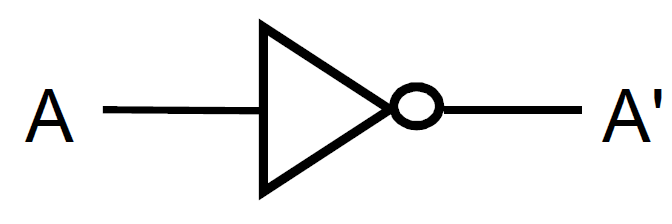
\includegraphics[width = 0.9\textwidth]{4_2.png}\end{minipage}&\begin{minipage}{3cm}\centering
\begin{tabular}{|c|c|}
\hline
$A$ & $A^\prime$
\\\hline
0 & 1
\\\hline
1 & 0
\\\hline
\end{tabular}
\end{minipage}\\\hline
\texttt{AND} Gate&\begin{minipage}{3cm}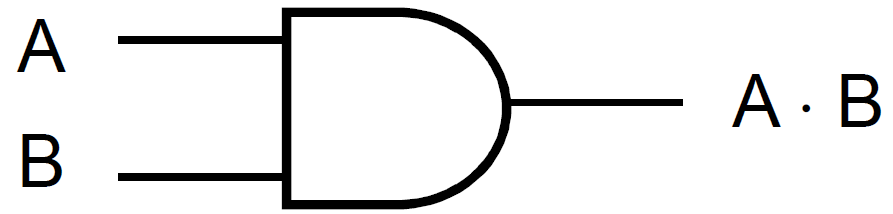
\includegraphics[width = 0.9\textwidth]{4_3.png}\end{minipage}&\begin{minipage}{3cm}\centering\begin{tabular}{|c|c|C{2cm}|}
\hline
$A$ & $B$ & $A\cdot B$
\\\hline
0 & 0 & 0
\\\hline
0 & 1 & 0
\\\hline
1 & 0 & 0
\\\hline
1 & 1 & 1
\\\hline
\end{tabular}
\end{minipage}\\
\hline
\texttt{OR} Gate&\begin{minipage}{3cm}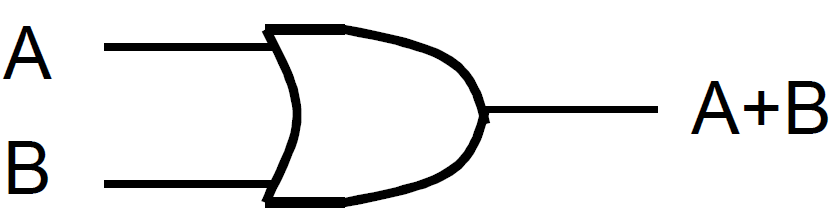
\includegraphics[width = 0.9\textwidth]{4_4.png}\end{minipage}&\begin{minipage}{3cm}\centering\begin{tabular}{|c|c|C{2cm}|}
\hline
$A$ & $B$ & $A+B$
\\\hline
0 & 0 & 0
\\\hline
0 & 1 & 1
\\\hline
1 & 0 & 1
\\\hline
1 & 1 & 1
\\\hline
\end{tabular}
\end{minipage}\\
\hline
\texttt{NAND} Gate&\begin{minipage}{3cm}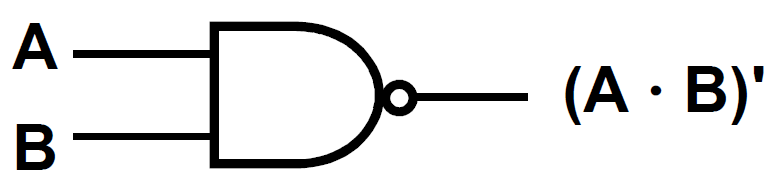
\includegraphics[width = 0.9\textwidth]{4_5.png}\end{minipage}&\begin{minipage}{3cm}\centering\begin{tabular}{|c|c|C{2cm}|}
\hline
$A$ & $B$ & $(A\cdot B)^\prime$
\\\hline
0 & 0 & 1
\\\hline
0 & 1 & 1
\\\hline
1 & 0 & 1
\\\hline
1 & 1 & 0
\\\hline
\end{tabular}
\end{minipage}\\
\hline
\texttt{NOR} Gate&\begin{minipage}{3cm}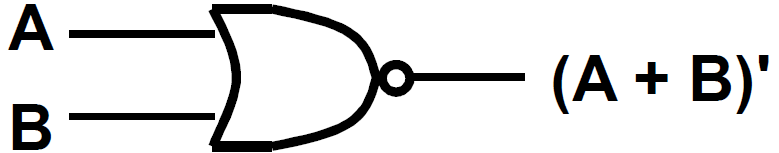
\includegraphics[width = 0.9\textwidth]{4_6.png}\end{minipage}&\begin{minipage}{3cm}\centering\begin{tabular}{|c|c|C{2cm}|}
\hline
$A$ & $B$ & $(A+B)^\prime$
\\\hline
0 & 0 & 1
\\\hline
0 & 1 & 0
\\\hline
1 & 0 & 0
\\\hline
1 & 1 & 0
\\\hline
\end{tabular}
\end{minipage}\\
\hline
\texttt{XOR} Gate&\begin{minipage}{3cm}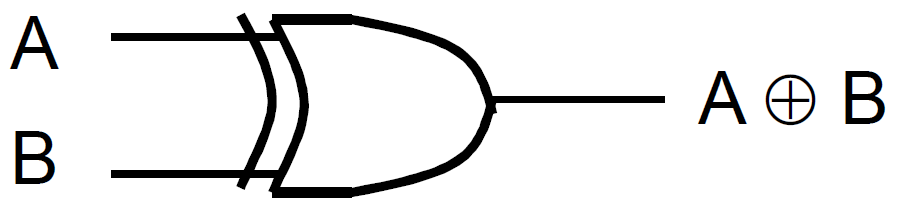
\includegraphics[width = 0.9\textwidth]{4_7.png}\end{minipage}&\begin{minipage}{3cm}\centering\begin{tabular}{|c|c|C{2cm}|}
\hline
$A$ & $B$ & $A\oplus B$
\\\hline
0 & 0 & 0
\\\hline
0 & 1 & 1
\\\hline
1 & 0 & 1
\\\hline
1 & 1 & 0
\\\hline
\end{tabular}
\end{minipage}\\
\hline
\texttt{XNOR} Gate&\begin{minipage}{3cm}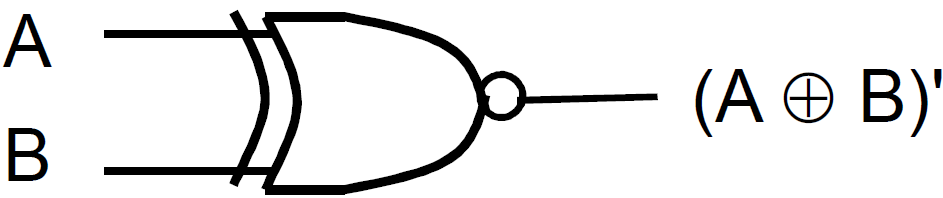
\includegraphics[width = 0.9\textwidth]{4_8.png}\end{minipage}&\begin{minipage}{3cm}\centering\begin{tabular}{|c|c|C{2cm}|}
\hline
$A$ & $B$ & $(A\oplus B)^\prime$
\\\hline
0 & 0 & 1
\\\hline
0 & 1 & 0
\\\hline
1 & 0 & 0
\\\hline
1 & 1 & 1
\\\hline
\end{tabular}
\end{minipage}\\
\hline
\end{tabular}
\end{table}
\clearpage
\subsection{Logic Circuit}
\begin{definition}[Fan-in]
\hfill\\\normalfont \textbf{Fan-in} refers to the number of inputs of a gate.
\end{definition}
Given a Boolean expression, we may implement it as a \textbf{logic circuit}.
\subsection{Universal Gates}
$\{\texttt{AND},\texttt{OR},\text{NOT}\}$ gates are sufficient for building any Boolean function. Thus the set $\{\texttt{AND},\texttt{OR},\text{NOT}\}$ is called a \textit{complete} set of logic.\\
However, other gates are also used for 
\begin{itemize}
  \item Usefulness
  \item Economical
  \item Self-sufficient
\end{itemize}
Furthermore, $\{\texttt{NAND}\}$ gate is a complete set of logic; $\{\texttt{NOR}\}$ gate is also a complete set of logic by duality.
\begin{figure}[h]
\begin{minipage}{0.1\textwidth}\texttt{NOT}\\\\\\\\\texttt{AND}\\\\\\\\\\\texttt{OR}
\end{minipage}\hfill
\begin{minipage}{ 0.4\textwidth}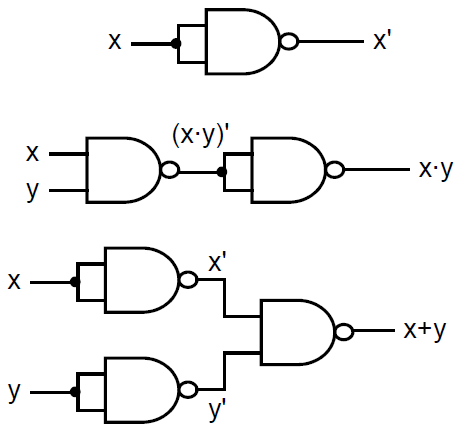
\includegraphics[width=\textwidth]{4_9.png}
\end{minipage}\hfill
\begin{minipage}{0.4\textwidth}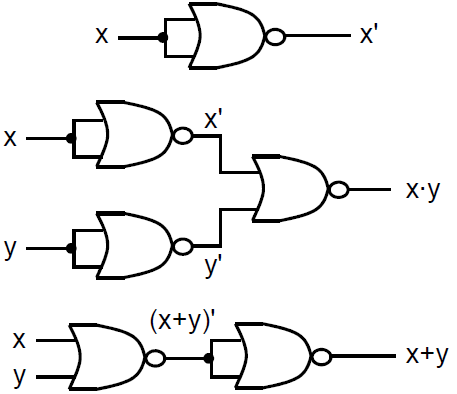
\includegraphics[width=\textwidth]{4_10.png}
\end{minipage}
\caption{Implementation of \texttt{OR}, \texttt{AND},\texttt{OR} using \texttt{NAND} and \texttt{NOR} respectively} 
\end{figure}
\subsubsection{SOP and \texttt{NAND} Circuits}
An SOP expression can be easily implemented using
\begin{itemize}
  \item 2-level \texttt{AND}-\texttt{OR} circuit
  \item 2-level \texttt{NAND} circuit
\end{itemize}
A 2-level \texttt{AND}-\texttt{OR} circuit can be converted to a 2-level \texttt{NAND} circuit by
\begin{enumerate}
  \item Introduce 2 \texttt{NOT} gate after first level \texttt{AND} and before second level \texttt{OR} gates.
  \item The first level \texttt{AND} have been converted to \texttt{NAND} gates; the second level negative-\texttt{OR} gate is \textit{equivalent} to \texttt{NAND} gate.
\end{enumerate} 
\subsubsection{POS and \texttt{NOR} Circuits}
A POS expression can be easily implemented using
\begin{itemize}
  \item 2-level \texttt{OR}-\texttt{AND} circuit
  \item 2-level \texttt{NOR} circuit
\end{itemize}
A 2-level \texttt{OR}-\texttt{AND} circuit can be converted to a 2-level \texttt{NOR} circuit by
\begin{enumerate}
  \item Introduce 2 \texttt{NOT} gate after first level \texttt{OR} and before second level \texttt{AND} gates.
  \item The first level \texttt{OR} have been converted to \texttt{NOR} gates; the second level negative-\texttt{AND} gate is \textit{equivalent} to \texttt{NOR} gate.
\end{enumerate} 
\clearpage
\section{Kaunaugh Map}
\textbf{Function simplification} leads to simpler expressions which uses fewer logic gates and makes circuits cheaper, less power consuming and faster.\\
There are three techniques in function simplification: Boolean Algebra, Karnaugh Maps and Quine-McCluskey.
\subsection{Boolean Algebra}
Algebraic simplification aims to minimise
\begin{itemize}
\item Number of literals, and
\item Number of terms
\end{itemize}
\subsection{Half Adder}
\begin{definition}[Half Adder]
\hfill\\\normalfont \textbf{Half adder} is a circuit that adds 2 single bits $(X,Y)$ to produce a result of 2 bits $(C,S)$.\footnote{$C$ is known as the carry bit, where $S$ is the sum bit.}\\
The truth table for half adder is
\begin{table}[h]
\centering
\begin{tabular}{|c|c||c|c|}
\hline
$X$ & $Y$ & $C$ &  $S$
\\\hline
0 & 0 & 0 & 0
\\\hline
0 & 1 & 0 & 1
\\\hline
1 & 0 & 0 & 1
\\\hline
1 & 1 & 1 & 0
\\\hline
\end{tabular}
\end{table}
\end{definition}
In canonical form (sum-of-minterms): 
\begin{itemize}
  \item $C=X\cdot Y$
  \item $S=X\cdot Y^\prime +X^\prime \cdot Y$ \footnote{In fact, $S=X\oplus Y$.}
\end{itemize}
The half adder can be implemented as 
\begin{figure}[h]\centering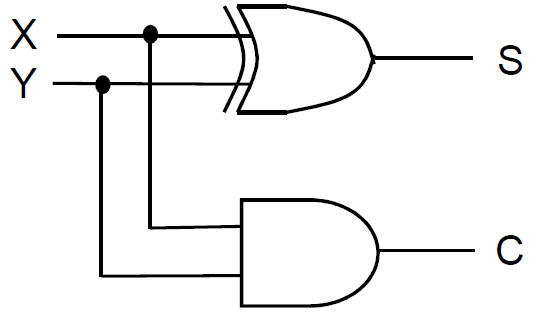
\includegraphics[width=0.3\textwidth]{4_11.png}\end{figure}
\clearpage
\subsection{Karnaugh Maps}
\textbf{Karnaugh Maps} is a systematic method to obtain simplified (minimal) sum-of-products(SOP) expressions. Its objective is to obtain \textit{fewest} produc terms and literals.
\begin{definition}[Kaunaugh Map]
\hfill\\\normalfont \textbf{Karnaugh Map} is an abstract form of Venn diagram, organised as a matrix of squares, where
\begin{itemize}
  \item Each square represents a minterm
  \item Two adjacent squares represent minterms that differ by \textit{exactly one} literal
\end{itemize}
\end{definition}
Layouts of Kaunaugh Maps from 2 variables to 6 variables are as following:
\begin{figure}[h]
\begin{minipage}{0.12\textwidth}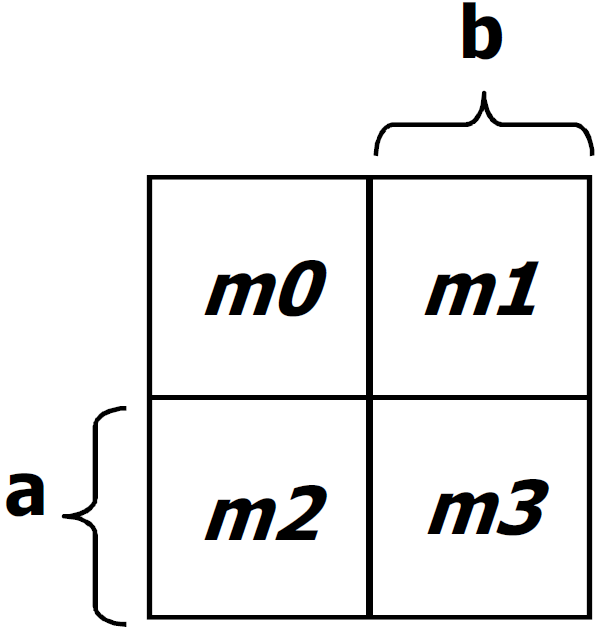
\includegraphics[width = \textwidth]{4_12.png}\end{minipage}\hfill
\begin{minipage}{0.35\textwidth}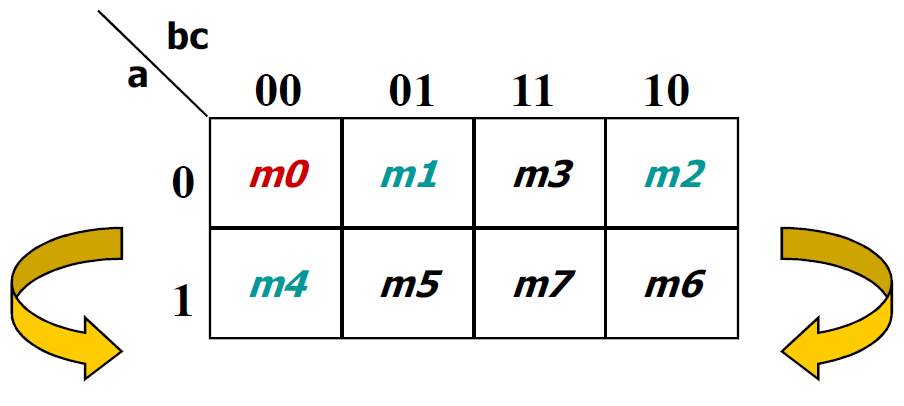
\includegraphics[width = \textwidth]{4_13.png}\end{minipage}\hfill
\begin{minipage}{0.43\textwidth}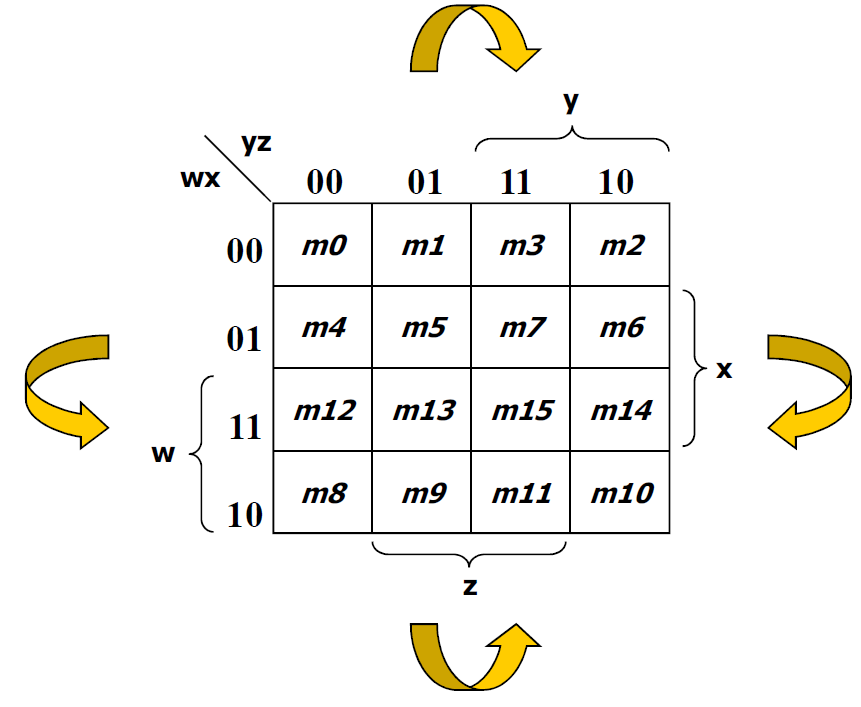
\includegraphics[width = \textwidth]{4_14.png}\end{minipage}\\
\begin{minipage}{0.49\textwidth}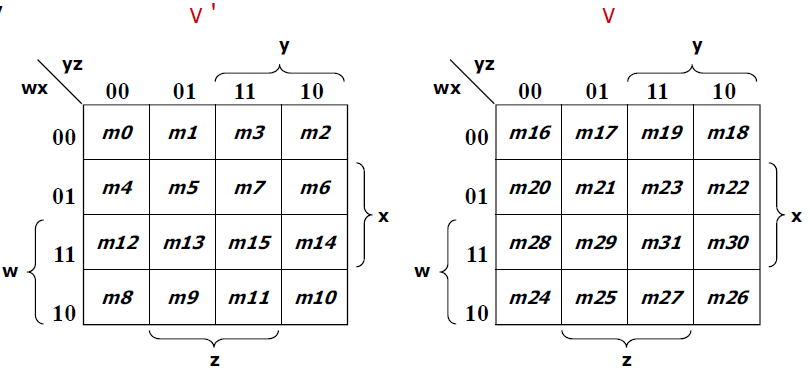
\includegraphics[width = \textwidth]{4_15.png}\end{minipage}\hfill
\begin{minipage}{0.49\textwidth}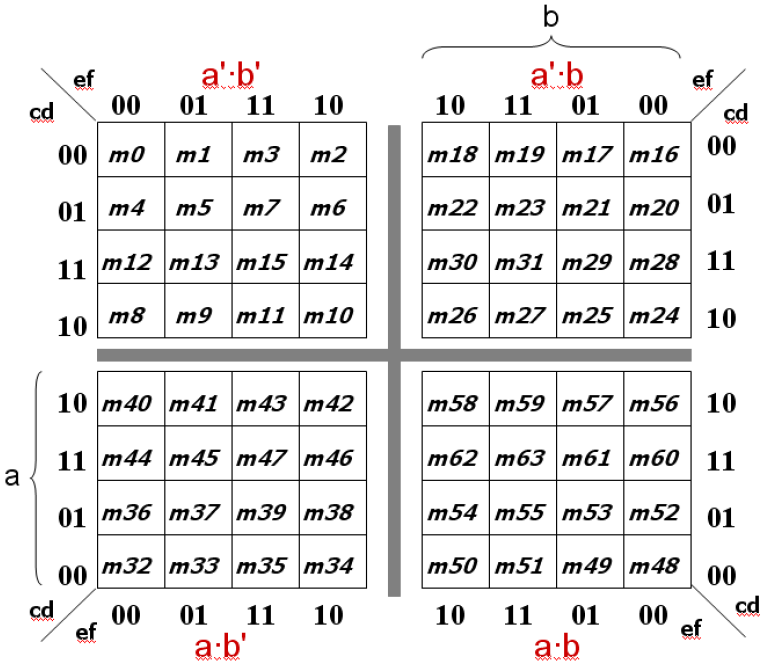
\includegraphics[width = \textwidth]{4_16.png}\end{minipage}

\end{figure}
Based on the \textbf{unifying theorem}
\[
A+A^\prime = 1
\]
In a K-map, each cell containing $1$ corresponds to a minterm of a given function $F$.\\
Each \textbf{valid grouping} of \textit{adjacent cells} containing 1 then corresponds to a \textbf{simpler product term} of $F$.
\begin{definition}[Valid Grouping]
\hfill\\\normalfont
\begin{itemize}
  \item A valid grouping admits a rectangular shape.
\item A valid grouping must have size in \textbf{powers of two}: $1,2,4,8,\ldots$.
\item Grouping $2^n$ adjacent cells eliminates $n$ variables.
\end{itemize}
\end{definition} 
In simplification, 
\begin{enumerate}
  \item Group as many cells as possible, by considering \textbf{prime implicants}.
  \item Select as few groups as possible to cover all the cells(minterms) of the function, by considering \textbf{essential prime implicants}.
\end{enumerate}
If a function is not in sum-of-minterms form,
\begin{itemize}
  \item Convert it into sum-of-products form
  \item Expand the SOP expression into sum-of-minterms expression.
\end{itemize}
\begin{definition}[Implicant]
\hfill\\\normalfont \textbf{Implicant} is a product term that could be used to cover minterms of the function.
\end{definition}
\begin{definition}[Prime Implicant]
\hfill\\\normalfont \textbf{Prime implicant} is a product term obtained by combining
the \textit{maximum} possible number of minterms from adjacent squares in the map.
\end{definition}
\begin{definition}[Essential Prime Implicant]
\hfill\\\normalfont \textbf{Essential Prime Implicant} is a prime implicant that includes at least one minterm that is not covered by any other prime implicant.
\end{definition}
\begin{theorem}[Algorithm for minimal SOP Expression]
\hfill\\\normalfont \begin{itemize}
\item Circle all prime implicants on the K-map.
\item Identify and select all essential prime implicants for the cover.
\item Select a minimum subset of the remaining prime implicants to complete the cover.\end{itemize}
\end{theorem}
\begin{theorem}[Algorithm for simplified POS Expression]
\hfill\\\normalfont \begin{itemize}
\item Group maxterms of $F$, equivalently minterms of $F^\prime$, identified as $9$ entry in K-map of $F$. This gives the SOP of $F^\prime$.\\
\item The simplified POS expression of $F$, use DeMorgan's law.
\end{itemize}
\end{theorem}
\begin{definition}[Don't care conditions]
\hfill\\\normalfont Outputs that can be either 1 or 0 are called \textbf{don't care conditions}, denoted by $X$.\\The set of don't care minterms are dentoed as $\sum d$.
\end{definition}
Don't care conditions can be used to help simplify Boolean expression further in K-maps.
\clearpage
\section{Combinatorial Circuits}
In combinatorial circuit, each output depends entirely on the immediate(present) input.
\subsection{Gate Level Design}
\begin{theorem}[Gate Level Design Procedure]
\begin{enumerate}
  \item State problems
  \item Determine and label the inputs and outputs of circuit
  \item Draw the truth table
  \item Obtain simplified Boolean functions.
  \item Draw logic diagram.
\end{enumerate} 
\end{theorem}
\subsubsection{Full Adder}
\textbf{Full adder} adds three bits $X,Y,Z$, which includes the carry, and output a sum bit $S$ and carry bit $C$.
\begin{figure}[h]
\centering
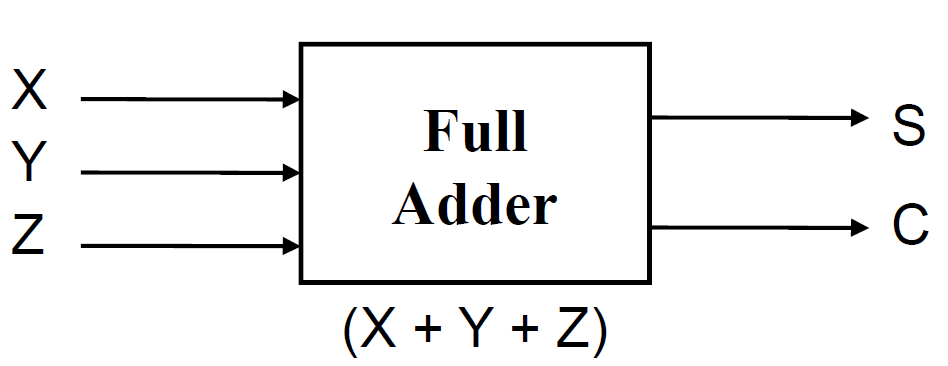
\includegraphics[width = 0.5\textwidth]{6_1.png}
\end{figure}
Truth table:
\begin{table}[h]
\centering
\begin{tabular}{|c|c|c||c|c|}
\hline
$X$&$Y$&$Z$&$C$&$S$\\\hline
0&0&0&0&0\\\hline
0&0&1&0&1\\\hline
0&1&0&0&1\\\hline
0&1&1&1&0\\\hline
1&0&0&0&1\\\hline
1&0&1&1&0\\\hline
1&1&0&1&0\\\hline
1&1&1&1&1\\\hline
\end{tabular}
\end{table}
Simplified formulae:
\begin{align*}
C&=X\cdot Y + (X\oplus Y)\cdot Z\\
S&=X\oplus(Y\oplus Z)
\end{align*}
Full Adder can be made from half adders.
\clearpage
\begin{figure}[ht]
\centering
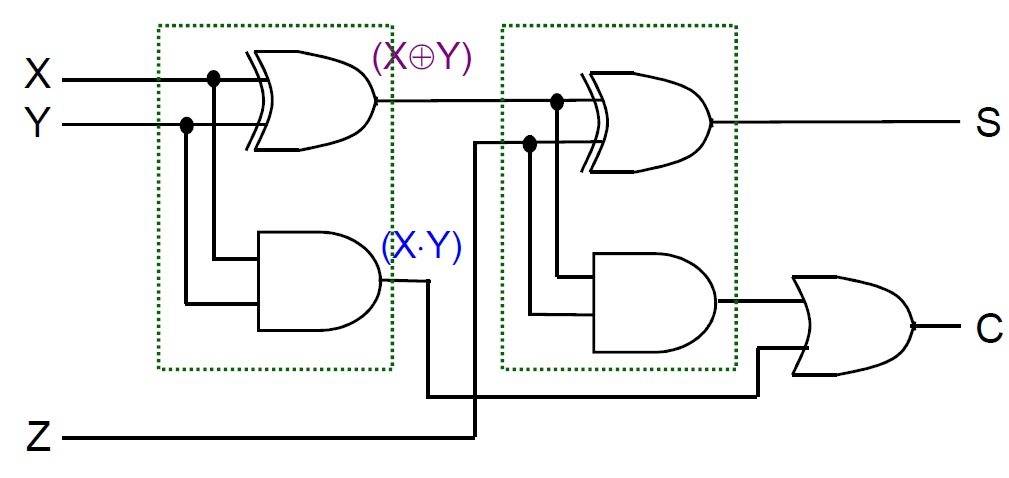
\includegraphics[width = 0.5\textwidth]{6_2.png}
\end{figure}
\subsection{Code Converters}
\begin{definition}[Code Converters]
\hfill\\\normalfont \textbf{Code converter} takes an input code and translates to its equivalent output code.
\end{definition}
\begin{figure}[h]
\centering
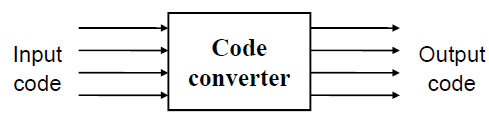
\includegraphics[width = 0.5\textwidth]{6_3.png}
\end{figure}
\begin{definition}[Binary Code Decimal]
\hfill\\\normalfont Binary code decimal is a representation system for coding a number in which each digit of a decimal number is represented individually by its binary equivalent.
\begin{table}[h]
\centering
\begin{tabular}{|c|c|}
\hline
Decimal digit&BCD\\\hline
0&0000\\\hline
1&0001\\\hline
2&0010\\\hline
3&0011\\\hline
4&0100\\\hline
5&0101\\\hline
6&0110\\\hline
7&0111\\\hline
8&1000\\\hline
9&1001\\\hline
\end{tabular}
\end{table}
\end{definition}
\begin{definition}[$f_\text{BCD}$]
\hfill\\\normalfont Let $(a_0a_1\ldots a_{n-1})_10$ be a decimal number. Its Binary Code Decimal is given by
\[
f_\text{BCD}(a_0a_1\ldots a_{n-1}) = s_{0,1}s_{0,2}s_{0,3}s_{0,4}\ldots s_{n-1,4}
\]
where $s_{i,1}s_{i,2}s_{i,3}s_{i,4}$ is the BCD of decimal $a_i$ defined from the truth table.
\end{definition}
As a result, the length of binary code decimal is always in multiple of 4.%
\subsection{Block Level Design}
Block level design method relies on algorithms or formulae of the circuit, which are obtained by decomposing the main problem to sub-problems recursively.
\subsubsection{4-bit adder}
Consider a circuit to add two 4-bit unsigned numbers together and a carry-in, to produced a 5-bit result.
\begin{figure}[h]
\centering
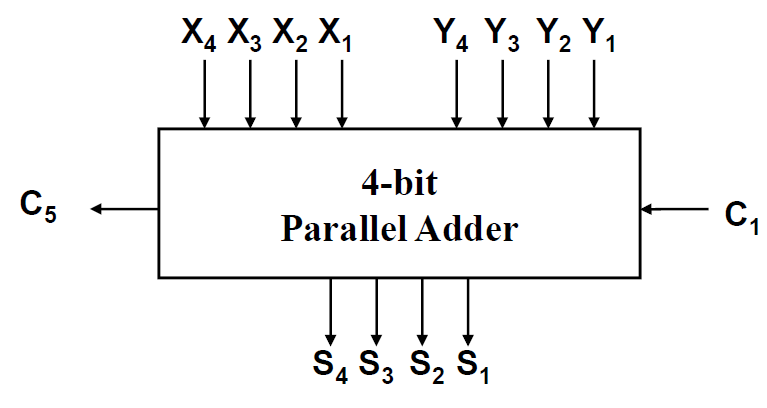
\includegraphics[width = 0.5\textwidth]{6_4.png}
\end{figure}
With the idea that $C_{i+1}S_i = X_i+Y_i +C_i$, which is the same function of full adder, 4-bit adder is implemented by cascading 4 full adders via their carries.
\begin{figure}[h]
\centering
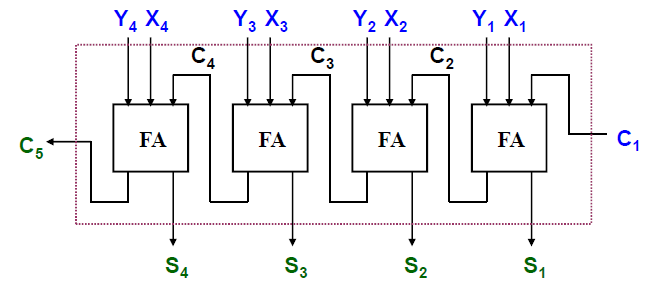
\includegraphics[width = 0.6\textwidth]{6_5.png}
\end{figure}
The above is called \textbf{parallel adder}, as inputs are presented in parallel.
\subsubsection{BCD-to-Excess-3 Converter}
Excess-3 code can be converted from BCD code using truth table. Therefore, gate-level design can be used since there are only 4 inputs. \\
However, alternative design is also possible, by identifying
\[
\text{Excess-}3\text{ code} = \text{BCD Code}+ 0011_2
\]
\clearpage
\begin{table}[h]
\centering
\begin{tabular}{|l|l|l|l|l|l|l|l|l|}
\hline
\multirow{2}{*}{} & \multicolumn{4}{l|}{BCD} & \multicolumn{4}{l|}{Excess-3} \\ \cline{2-9} 
                  & A    & B    & C    & D   & W     & X     & Y     & Z     \\ \hline
0                 & 0    & 0    & 0    & 0   & 0     & 0     & 1     & 1     \\ \hline
1                 & 0    & 0    & 0    & 1   & 0     & 1     & 0     & 0     \\ \hline
2                 & 0    & 0    & 1    & 0   & 0     & 1     & 0     & 1     \\ \hline
3                 & 0    & 0    & 1    & 1   & 0     & 1     & 1     & 0     \\ \hline
4                 & 0    & 1    & 0    & 0   & 0     & 1     & 1     & 1     \\ \hline
5                 & 0    & 1    & 0    & 1   & 1     & 0     & 0     & 0     \\ \hline
6                 & 0    & 1    & 1    & 0   & 1     & 0     & 0     & 1     \\ \hline
7                 & 0    & 1    & 1    & 1   & 1     & 0     & 1     & 0     \\ \hline
8                 & 1    & 0    & 0    & 0   & 1     & 0     & 1     & 1     \\ \hline
9                 & 1    & 0    & 0    & 1   & 1     & 1     & 0     & 0     \\ \hline
10                & 1    & 0    & 1    & 0   & X     & X     & X     & X     \\ \hline
11                & 1    & 0    & 1    & 1   & X     & X     & X     & X     \\ \hline
12                & 1    & 1    & 0    & 0   & X     & X     & X     & X     \\ \hline
13                & 1    & 1    & 0    & 1   & X     & X     & X     & X     \\ \hline
14                & 1    & 1    & 1    & 0   & X     & X     & X     & X     \\ \hline
15                & 1    & 1    & 1    & 1   & X     & X     & X     & X     \\ \hline
\end{tabular}
\end{table}
\begin{figure}[h]
\centering
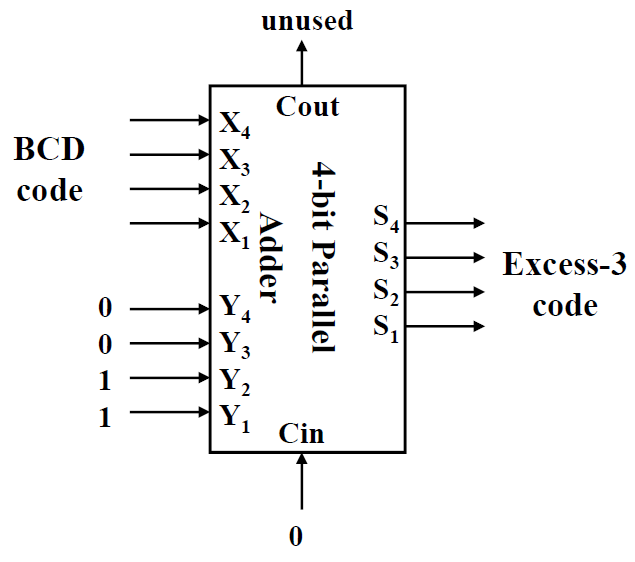
\includegraphics[width = 0.4\textwidth]{6_6.png}
\caption{BCD-to-Excess-3 Code Converter}
\end{figure}
\subsubsection{16-bit Parallel Adder}
Larger parallel adders can be built from smaller ones.\\A \textbf{16-bit parallel adder} can be contructed from four 4-bit parallel adders:
\clearpage
\begin{figure}[h]
\centering
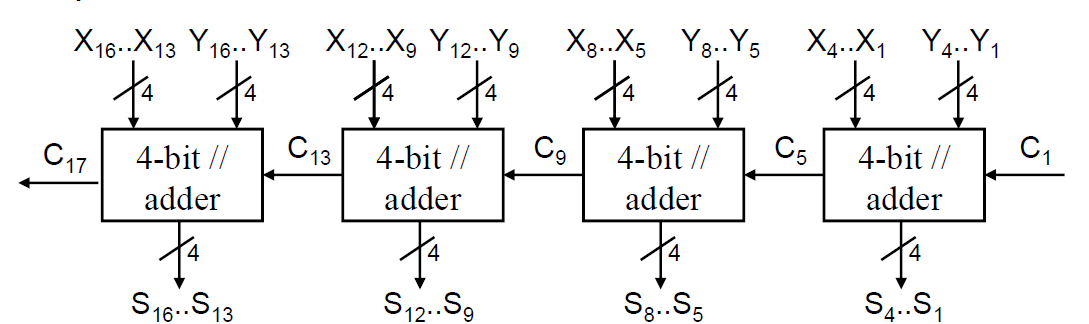
\includegraphics[width = 0.8\textwidth]{6_7.png}
\end{figure}
\subsubsection{4-bit Adder cum Subtractor}
\textbf{4-bit Adder cum Subtractor} is a circuit that can perform both addition and subtraction, using a parallel adder with a control signal.\\
Recall
\begin{align*}
X-Y &=X+(-Y)\\
&=X+\text{2s complement of }Y\\
&=X+\text{1s complement of }Y + 1
\end{align*}
Therefore, \texttt{XOR} gates are used to flip bits\footnote{Note $x$\texttt{ XOR }0 = $x$, and $x$\texttt{ XOR }1 = $x^\prime$} and control signal $S$ is connected to input carry-in.
\begin{figure}[h]
\centering
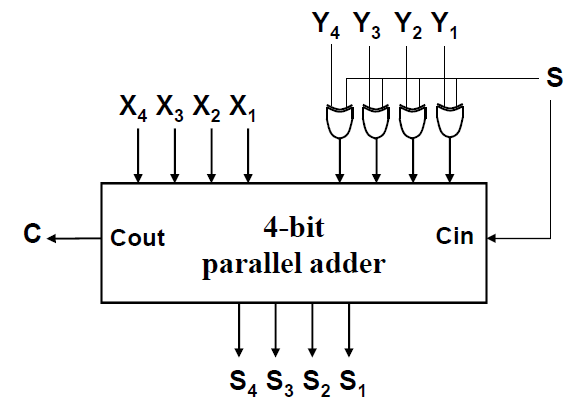
\includegraphics[width = 0.8\textwidth]{6_9.png}
\end{figure}
\clearpage
When $S=1$, it it subtracts by adding $X$ with $Y^\prime$ and $S=1$, and when $S=0$, it adds by adding $X$ with $Y$ with $S=0$.
\subsubsection{Magnitude Comparator}
\textbf{Magnitude comparator} compares 2 values $A$ and $B$, to output either $A>B$, $A=B$ or $A<B$.\\The key idea is that $X\cdot Y^\prime$ outputs 1 when $X>Y$ and 0 otherwise. Therefore, $X=Y$ if and only if $(X\cdot Y^\prime)\texttt{ NOR }(X^\prime \cdot Y) = X\cdot Y + X^\prime \cdot Y^\prime= 1$.\\
We first build a 4-bit magnitude comparator using the above logic. Let $A=A_3A_2A_1A_0$, $B = B_3B_2B_1B_0$. Denote $x_i = A_i\cdot B_i + A_i^\prime\cdot B_i^\prime$.
\begin{figure}[h]
\centering
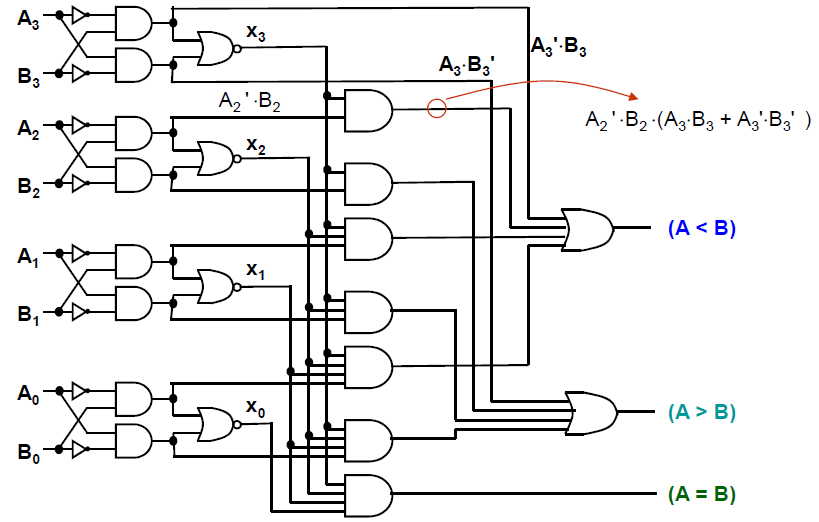
\includegraphics[width = 0.7\textwidth]{6_10.png}
\end{figure}
This generates the block diagram of 4-bit magnitude comparator
\begin{figure}[h]
\centering
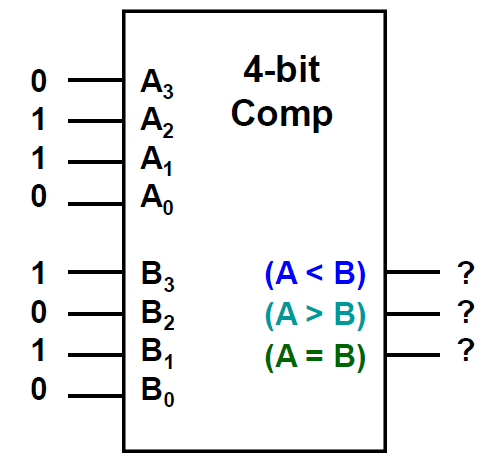
\includegraphics[width = 0.5\textwidth]{6_11.png}
\end{figure}
\subsection{Circuit Delays}
\begin{definition}[Circuit Delay]
\hfill\\\normalfont Given a logic gate with delay $t$. If inputs are stable at times $t_1,\ldots, t_n$, then the earliest time in which the output will be stable is
\[
\max(t_1,\ldots, t_n)+t
\]
\end{definition}
Suppose a full adder has delay $t_1,t_2$ for $X,Y$ and $t_3$ for carry in, $S$ will have delay \[ S_\text{delay} = \max\{\max\{t_1+t_2\}+t,t_3 \}+t\]
$C$ will have delay \[
C_\text{delay} = \max\{\max\{t_1,t_2\}+t,t_3\}+2t
\] 
According to the above, a $n$-bit ripple-carry parallel adder will experience the following delay\footnote{$n$ is of index 1.}
\begin{align*}
S_n &= 2nt\\
C_{n+1}&=(2n+1)t
\end{align*}
Therefore, propagation delay of ripple-carry parallel adders is proportional to the number of bits it handles.
\subsubsection{Carry Look-ahead Adder}
\begin{figure}[h]
\centering
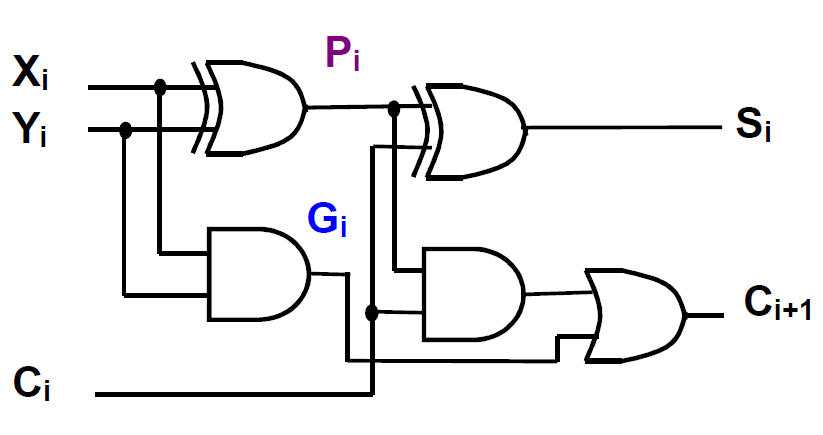
\includegraphics[width = 0.5\textwidth]{6_12.png}
\end{figure}
Consider the full adder, define intermediate signals $P_i,G_i$ as follows
\begin{align*}
P_i&=X_i\oplus Y_i\\
G_i = X_i\cdot Y_i
\end{align*}
Therefore, the output $S_i, C_{i+1}$ can be given in terms of $C_i,P_i,G_i$:
\begin{align*}
S_i &= P_i\oplus C_i\\
C_{i+1}&=G_i+P_i\cdot C_i\;\;\;\;\;(\#)
\end{align*}
We can regard, $G_i$ as the \textbf{carry generate} signal, since $G_i = 1$ suggests both $X_i$ and $Y_i$ is 1, which definitely \textit{generates} a carry $C_{i+1}=1$.\\

Also, $P_i$ can be regarded as the \textbf{carry propagate} signal, as $P_i= 1$ suggests exactly $X_i=1$ or $ Y_i = 1$ but not both. Therefore, $C_{i+1} = 1$ if $C_i = 1$ and $P_i = 1$, which suggests that the status of carry in $C_i$ is \textit{propagated} to carry out $C_{i+1}$.\\

For the 4-bit ripple carry adder, the equation for $C_{i+k}, k = 1,\ldots, 4$ is only dependent on $G_j,P_j,C_j, 1\leq j< i+k$, according to the recursively relation $(\#)$. 
By expanding the recursive relation into an iterative expression we have
\[
C_{i+k}=\prod_{j=0}^{k-1} P_j\cdot C_i+\sum_{j=0}^{k-1}G_{i+j}\prod_{l = j+1}^{k-1}P_{i+l}
\]
which is a two level sum of product expressions in terms of $G,P,C$.\\
\begin{figure}[h]
\centering
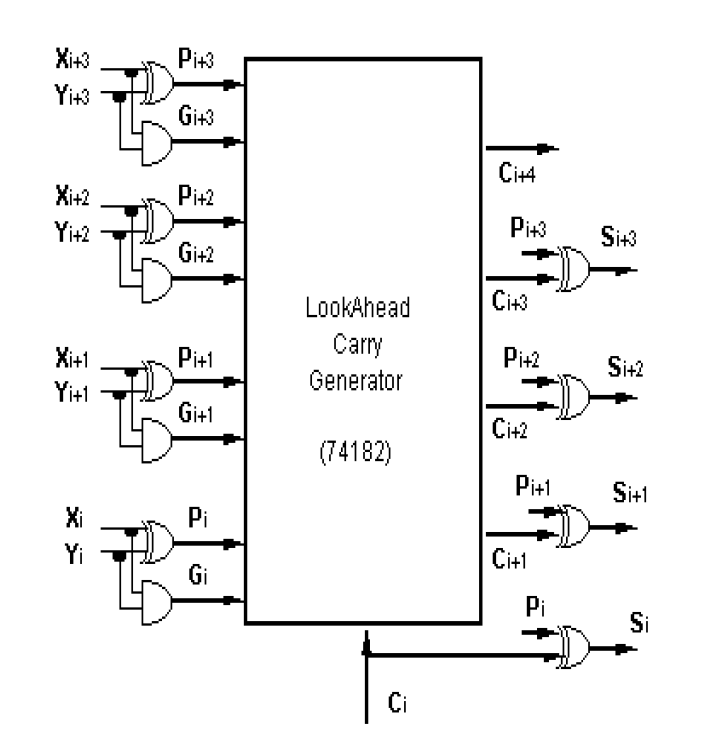
\includegraphics[width = 0.5\textwidth]{6_14.png}
\caption{$X_i,Y_i$ are preprocessed outside the block. Block inputs $P,G$ only and outputs $C$ only.}
\end{figure}

The generation of $P,G$ of each bit takes time $t$ from \texttt{XOR} and \texttt{AND} gate; generation of each carry $C_{i+k}$ takes time $2t$ from the sum of product expression; generation of sum signals $S_{i+k}$ of each bit takes time $t$ from $P_{i+k},C_{i+k-1}$. Therefore, the whole process takes time $4t$.\\

Larger block carry look-ahead adder can be built from 4-bit carry look-ahead adder. Two \textit{additional} output is needed: \textbf{block carry generate} and \textbf{block carry propagate}.\\

Let $P_0,P_1,P_2,P_3$ be the 4 carry propagate bits of the 4-bit carry look-ahead adder. Let $G_0,G_1,G_2,G_3$ be the 4 carry generate bits of the 4-bit carry look-ahead adder. Then the \textbf{block} carry propagate and generate bits, $P^\ast $ and $G^\ast$, respectively are defined as
\begin{align*}
P^\ast = P_0\cdot P_1\cdot P_2\cdot P_3\\
G^\ast = G_3+G_2\cdot P_3+G_1\cdot P_2\cdot P_3+G_0\cdot P_1\cdot P_2\cdot P_3
\end{align*}
It is easy to see that the carry out bit of block 4-bit carry look-ahead adder is 
\[
C_3 = G^\ast +P^\ast\cdot C_{-1}
\]
where $C_{-1}$ is the carry in to the 4-bit block.
\begin{figure}[h]
\centering
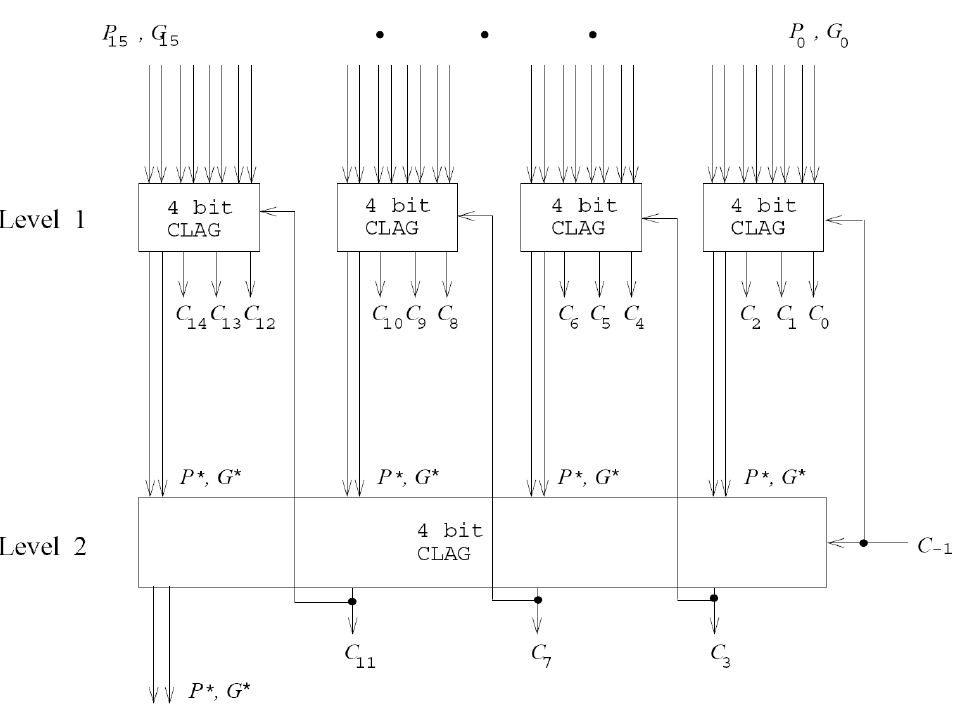
\includegraphics[width = 0.9\textwidth]{6_13.png}
\end{figure}
The sequence of availability of output is that
\begin{itemize}
  \item Time 0: $P_0\sim P_{15},G_0\sim G_{15}, C_{-1}$.
  \item Time 1: $C_0\sim C_2$, all $P^\ast, G^\ast$ between level 1 and level 2.
  \item Time 2: $C_4,C_7,C_11,P^\ast,G^\ast$ after level 2
  \item Time 3: Rest $C_4\sim C_{14}$.\footnote{$C_4$ is dependent on $C_3$, which is dependent on $P^\ast and G^\ast$, which is dependent on $P,G$.}
\end{itemize}
\clearpage
\section{More Building Blocks}
\subsection{Decoder}
\begin{definition}[Decoder]
\hfill\\\normalfont A \textbf{decoder} converts binary information from $n$ input lines to $2^n$ output lines.
\end{definition}
\subsubsection{Truth table}
The truth table for $2^n$ output, when input is enumerated in increasing sequence, is diagonal. The column of output is arranged according to the increasing order of minterm of the function.\\

\begin{theorem}[Building functions using decoder]\hfill\\\normalfont
Any boolean function with $n$ input with $m$ output can be built using a $n:2^n$ decoder, which generates the minterms, and $m$ \texttt{OR} gates to form the sum.
\end{theorem}

Decoders often come with an \textbf{enable control} signal, so that the device is only activated when the enable $E = 1$. \\
\begin{figure}[h]
\centering
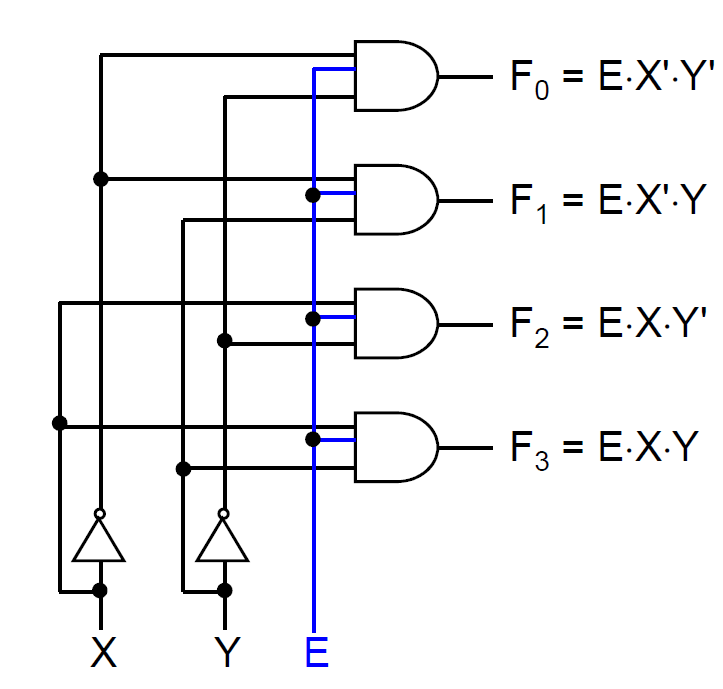
\includegraphics[width = 0.5\textwidth]{7_1.png}
\caption{Implementation of 2:4 Encoder with \textbf{one-enable} control $E=1$}
\end{figure}
In most MSI decoders, enable signal is \text{zero-enable}, usually denoted by $E^\prime$. The decoder is enabled when signal $E$ is low.\\
\subsubsection{Larger Decoder}
Larger decoders can be constructed, with one inverter from smaller ones by treating $E$ as the most significant bit which selects the smaller decoders.
\subsubsection{Implementing functions}
We may implement the functions using a decoder in several ways.\\Suppose a function is specified as $f(A,B,C) = \sum m(0,1,4,6,7) = \prod M(2,3,5)$, we may implement it 
\begin{itemize}
  \item using a decoder with active high outputs\footnote{Given any input, only one of the output will be 1 and rest 0} with a \texttt{OR} gate on minterms:
  \[
f = m_0+m_1+m_4+m_6+m_7
  \]
  \item using a decoder with active low outputs\footnote{Given any input, only one of the output will be 0 and rest 1} with a \texttt{NAND} gate on minterms:
  \[
f = (m_1^\prime\cdot m_2^\prime\cdot m_4^\prime\cdot m_6^\prime\cdot m_7^\prime)^\prime
  \]
  \item Using a decoder with active high outputs with a \texttt{NOR} gate on maxterms:
  \[
f = (m_2+m_3+m_5)^\prime
  \]
  \item Using a decoder with active low outputs with a \texttt{AND} gate on maxterms:
  \[
f = m_2^\prime\cdot m_3^\prime\cdot m_5^\prime
  \]
\end{itemize}
\subsection{Encoders}
\begin{definition}[Encoder]
\hfill\\\normalfont Given $2^n$ input lines, of which \textit{exactly} 1 is high, the \textbf{encoder} provides a $n$ bit code that corresponds to that input line.
\end{definition}
\begin{figure}[h]
\centering
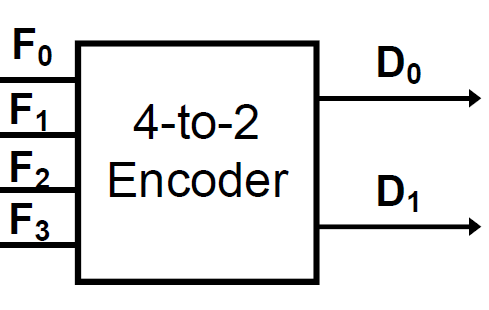
\includegraphics[width = 0.4\textwidth]{7_7.png}
\end{figure}
\subsubsection{Truth Table}
For the truth table of an encoder, when exactly 1 out of $2^n$ inputs is high, say $F_i$, the output $D_n D_{n-1}\cdots D_1 D_0$ is the binary string $i_2$; if more than 1 input are high, the output becomes don't care.
\clearpage
\begin{figure}[h]
\centering
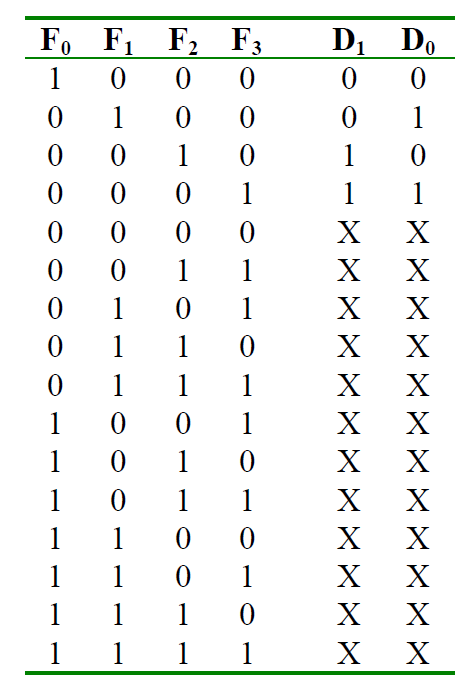
\includegraphics[width = 0.4\textwidth]{7_2.png}
\caption{$D_0 = F_1+F_3$, $D_1 = F_2+F_3$}
\end{figure}
The implementation of a specified output is the sum of inputs whose specified output are high, given the benefits of don't cares. \\Therefore, encoders can be designed using \texttt{OR} gate.
\subsubsection{Priority Encoder}
In priority encoder, each of the inputs is assigned a \textbf{priority}.\\The \textbf{most} significant bit of the input has the \textbf{highest} priority while the least significant bit has the lowest priority.

If two input lines goes high, only the \textit{higher} priority one will be considered as high. This generates a truth table with don't cares in inputs.
\begin{figure}[h]
\centering
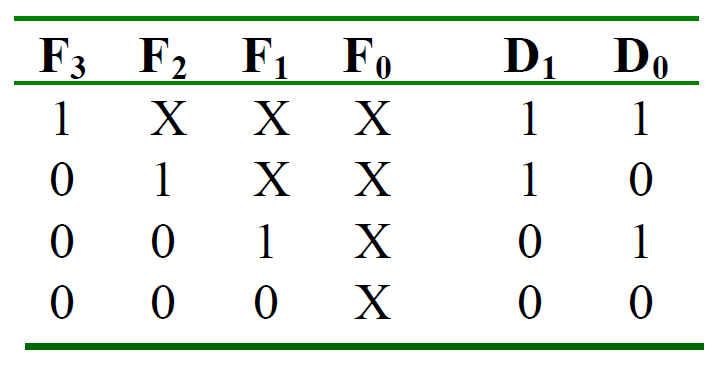
\includegraphics[width = 0.4\textwidth]{7_3.png}
\caption{Truth table of priority encoder}
\end{figure}

\subsection{Demultiplexers}
\begin{definition}[Demultiplexers]
\hfill\\\normalfont Given an input line and a set of $n$ selection lines, a \textbf{demultiplexer} directs data from the input to \textit{one} selected output line out of $2^n$.
\end{definition}
Suppose the selection lines admits a $N=(S_{n-1}\ldots S_0)_2$ binary number, the output line $Y_N$ will correspondingly be selected such that $Y_N = D$, the input.
\begin{figure}[h]
\centering
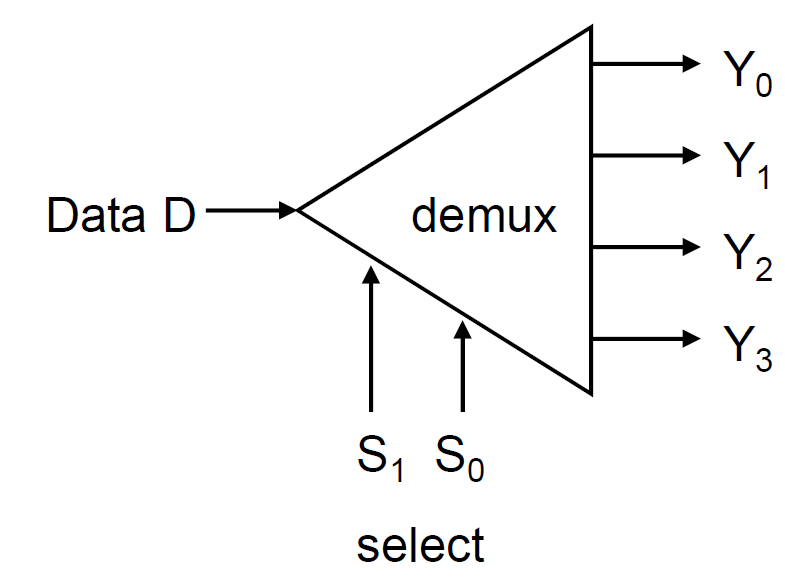
\includegraphics[width = 0.5\textwidth]{7_4.png}
\end{figure}
\subsubsection{Truth Table}
The truth table for outputs from demultiplexers of $n$ selection lines, when the selection lines is enumerated in increasing sequence, is diagonal $D$, where $D$ is the input.\\There is similarity of truth table between demultiplexers and decoders. In fact,a demultiplexer of $n$ selection line can be implemented using a $n:2^n$ decoder with selection lines connected to the input of decoders and data input connected to the enable bit.
\begin{figure}[h]
\centering
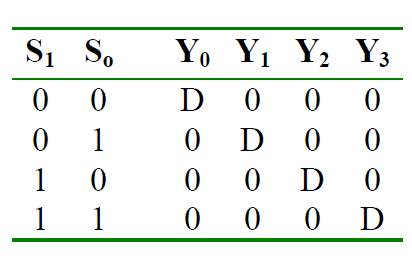
\includegraphics[width = 0.4\textwidth]{7_5.png}
\end{figure}
\subsection{Multiplexers}
\begin{definition}[Multiplexers]
\hfill\\\normalfont A \textbf{multiplexer} is a device with has $2^n$ input lines, $n$ selection lines and 1 output line. It steers one of $2^n$ inputs to a single output line.
\begin{figure}[h]
\centering
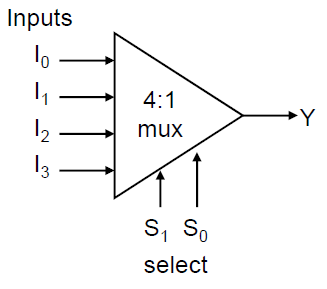
\includegraphics[width = 0.4\textwidth]{7_6.png}
\end{figure}
\end{definition}
\subsubsection{Truth Table}
The output $Y$ equals to $I_i$, the $i$th input, where binary representation of $i$ equals to the binary string given by selection lines $S_{n-1}\ldots S_0$.\\
Therefore, a $2^n:1$ multiplexer can be made from connecting selection lines to an $n:2^n$ decoder and adding the $2^n$ output to the $2^n$ input lines, each with \texttt{AND} gate, and \texttt{OR} the $2^n$ processed input.
\begin{figure}[h]
\centering
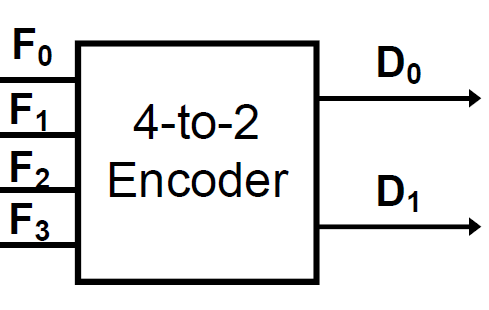
\includegraphics[width = 0.4\textwidth]{7_7.png}
\end{figure}
It is also common to see enable bit in multiplexers.
\subsubsection{Larger Multiplexers}
Larger multiplexers can be constructed from smaller ones, by seperating selection lines into multiple hierarchies of multiplexers.
\subsubsection{Implementing functions}
Just like decoder, Boolean functions can be implemented using multiplexers. Specifically, a $2^n:1$ multiplexer can implement a Boolean function of $n$ input variables, as follows:
\begin{itemize}
  \item Express in sum-of-minterms form.
  \item Connect $n$ variables to the $n$ selection lines.
  \item Put a $1$ on data input if it is a minterm of the function or $0$ otherwise.
\end{itemize}
A Boolean function of $n$ input variables can be implemented by a smaller $2^{n-1}:1$ multiplexer.
\begin{itemize}
  \item Express Boolean function in sum-of-minterms form
  \item Reserve one variable for input lines and use the rest for selection lines.
  \item se a truth table and deduce multiplexer input by comparing the reserved variable and the function value for corresponding selection line values. It may take $1, 0, V, V^\prime$, one of the four possibilities.
\end{itemize}
\subsection{Carry-select Adders}
Carry-Select Adders reduce waiting time of the carry chain by divide-and-conquer using multiplexers.

To add two $n$-bit numbers $A$ and $B$ to produce the result $C$, split $A, B, C$ into two equal halves: $A_H A_L, B_H, B_L, C_H,C_L$.\footnote{$H$ stands for high, $L$ stands for low.}
\begin{figure}[h]
\centering
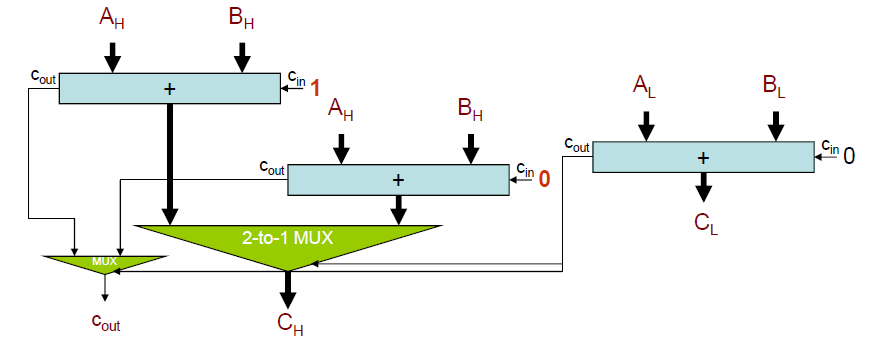
\includegraphics[width = \textwidth]{7_9.png}
\end{figure}
The idea is that the addition of $A_L + B_L$ will either has a carry or not, so it computes the two scenarios for $A_H+B_H+c$ along with $A_L+B_L$, and the carry out $c$ from $A_L+B_L$ will select the final carry out and $C_H$.
\subsection{Shifters}
Shifting is a common operation, as left shift by 1 bit is equivalent to multiplying by 2, and right shift by 1 bit is equivalent to dividing by 2, for positive numbers.
\subsubsection{Arithmetic Shift}
In arithmetic left shift, $0$ is used to fll in the LSB.\\
In arithmetic right shift, the original MSB is duplicated at MSB; for 2's complement, only the part other than the sign bit is shifted.
\subsubsection{Barrel Shifters}
Barrel Shifters perform fast shifting in $O(\log n)$ time by always shifting in the power of $2$. \footnote{Shifting by 11 is performed by shifting $8+2+1$, a total of 3 times.}
The fast shifting is implemented using multiplexers.
\begin{figure}[h]
\centering
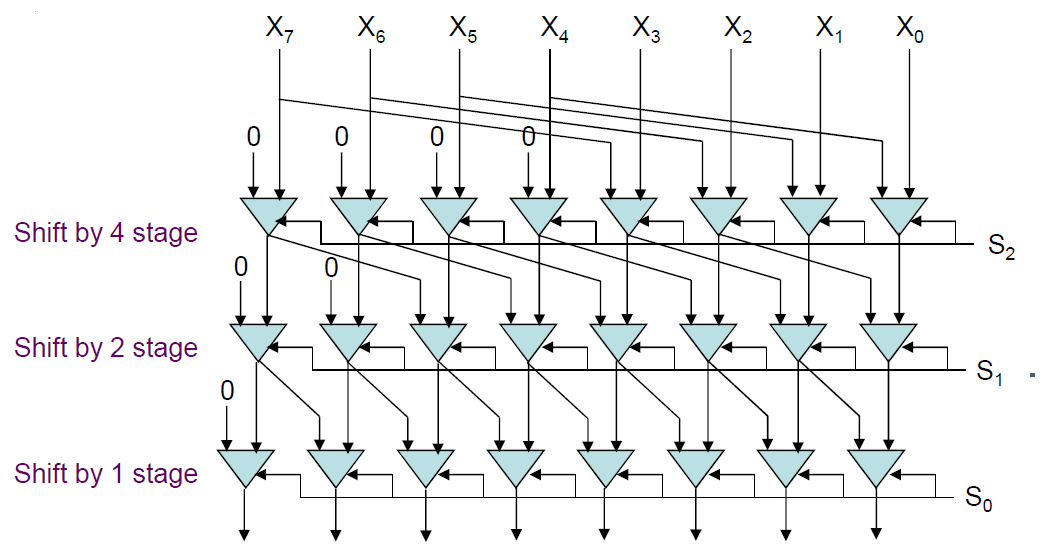
\includegraphics[width = 0.8\textwidth]{7_10.png}
\end{figure}
At each shifting stage, the selection line $S_k$, calculated from the amount of total shifts, we decide whether to shift by $2^k$ bits or remain unchanged. 
\clearpage
\section{Sequential Logic}
There are two types of sequential circuits:
\begin{itemize}
  \item \textbf{Synchronous}: outputs change only at specific time
  \item \textbf{Asynchronous}: outputs change at any time
  \end{itemize}
\begin{definition}[Finite State Machines]
\hfill\\\normalfont \textbf{Finite State Machines} are built with combinatorial logic and \textbf{memory}, which stores the state. \\Next state depends on current state and inputs. 
\end{definition}
\subsection{$S-R$ Latch}
$S-R$ latch consists of two \textbf{inputs} $S$ and $R$, stands for SET and RESET respectively.\\It has two \textbf{complementary output} $Q$ and $Q^\prime$. $Q=1\Leftrightarrow$ latch is in SET state; $Q=0\Leftrightarrow$ latch is in RESET state.
\subsubsection{Characteristic Table}
\begin{table}[h]
\centering
\begin{tabular}{|c|c|c|c|c|}
\hline
$S$&$R$&$Q$&$Q^\prime$&\\\hline
0&0&NC&NC&No change to present state\\\hline
1&0&1&0&Latch SET\\\hline
0&1&0&1&Latch RESET\\\hline
1&1&0&0&Invalid Condition\\\hline
\end{tabular}
\end{table}
From this table, we have $Q(t+1) = S+R^\prime\cdot Q(t)$, with restriction $S\cdot R = 0$.\\
The implementation of $S-R$ latch is as follows
\begin{figure}[h]
\centering
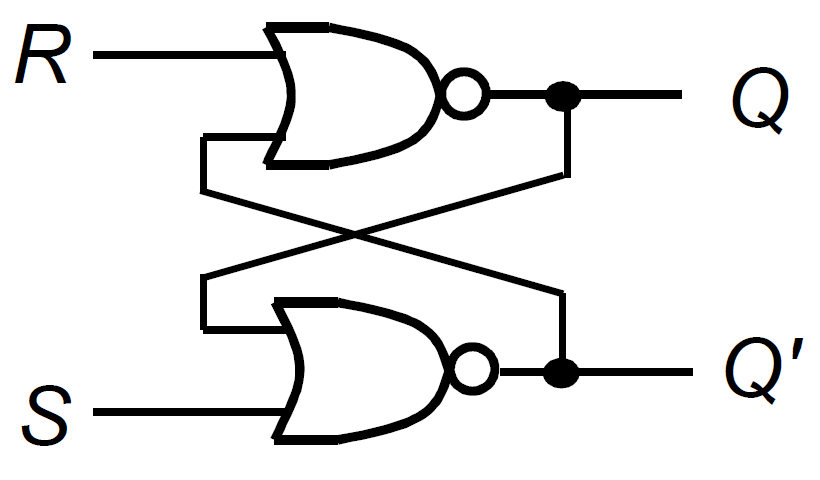
\includegraphics[width = 0.3\textwidth]{8_1.png}
\end{figure}
A $S-R$ latch is gated if it has an enable input($EN$). Its output will change only when $EN$ is high. Its implementation becomes\footnote{Note the position of $S$ and $R$ relative to $Q$}
\clearpage
\begin{figure}[h]
\centering
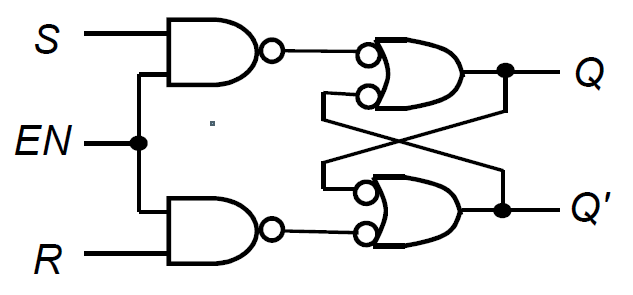
\includegraphics[width = 0.5\textwidth]{8_2.png}
\end{figure} 

\subsection{Gated $D$ Latch}
If $D:=S$ and $R:=S^\prime = D^\prime$, a gated $S-R$ latch becomes a gated $D$ latch.\\$D$ latch eliminates the invalid state by admitting the following characteristic table
\begin{table}[h]
\centering
\begin{tabular}{|c|c|c|c|}
\hline
$EN$&$D$&$Q(t+1)$&\\\hline
1&0&0&RESET\\\hline
1&1&1&SET\\\hline
0&X&$Q(t)$&No change\\\hline
\end{tabular}
\end{table}
Hence, when $EN = 1$, $Q$ follows $D$ input in a sense $Q(t+1) = D$, and when $EN = 0$, $Q(t+1) = Q(t)$.
\subsection{Flip-flops}
\begin{definition}[Flip-flops]
\hfill\\\normalfont \textbf{Flip-flops} are \textbf{synchronous bistable} devices. Output changes state at a specified point on a triggering input called the \textbf{clock}. 
\end{definition}
Flip-flops change state eigher at the positive edge or at the negative edge of the clock signal. \\
Flip-flop family has $S-R$ flip-flop, $D$ flip-flop and $J-K$ fllip-flop.
\begin{figure}[h]
\centering
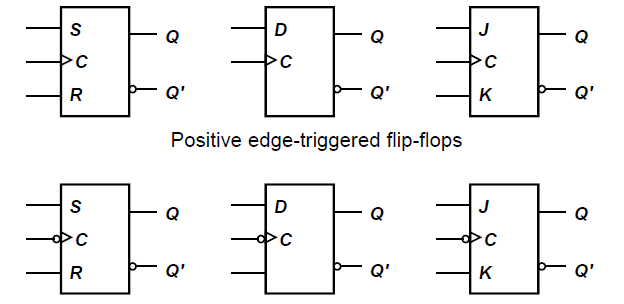
\includegraphics[width = 0.5\textwidth]{8_3.png}
\end{figure} 
\subsection{$S-R$ flip-flop}
$S-R$ flip-flop has the only difference from the $S-R$ latch in that its output changes onlyon the triggering edge of the clock pulse.\\Its characteristic table is

\clearpage\begin{table}[h]
\centering
\begin{tabular}{|c|c|c|c|c|}
\hline
$S$&$R$&$CLK$&$Q(t+1)$&\\\hline
0&0&X&$Q(t)$&No change\\\hline
0&1&$\uparrow$&0&RESET\\\hline
1&0&$\uparrow$&1&SET\\\hline
1&1&$\uparrow$&?&Invalid\\\hline
\end{tabular}
\end{table}
\subsection{$D$ flip-flop}
$D$ flip-flop has single input $D$ and is similar to gated $D$ latch. Its characteristic table is
\begin{table}[h]
\centering
\begin{tabular}{|c|c|c|c|}
\hline
$D$&$CLK$&$Q(t+1)$&\\\hline
1&$\uparrow$&1&SET\\\hline
0&$\uparrow$&0&RESET\\\hline
\end{tabular}
\end{table}
$D$ flip-flop is useful in parallel data transfer.
\subsection{$J-K$ flip-flop}
$J-K$ flip-flop is an enhancement of $S-R$ flip-flop($J:=S, K:=R$) by replacing the invalid state($S=1, R=1$) by a \textbf{toggle} state, at which $Q(t+1) = Q(t)^\prime$.\\
$J-K$ flip-flop is achieved by feeding $Q$ and $Q^\prime$ to the pulse steering NAND gates.
\begin{figure}[h]
\centering
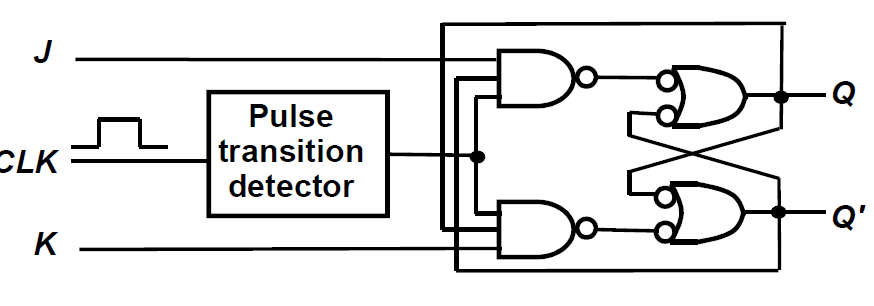
\includegraphics[width = 0.7\textwidth]{8_4.png}
\end{figure}\\
It admits the following characteristic table:\clearpage
\begin{table}[h]
\centering
\begin{tabular}{|c|c|c|c|c|}
\hline
$J$&$K$&$CLK$&$Q(t+1)$&\\\hline
0&0&$\uparrow$&$Q(t)$&No change\\\hline
0&1&$\uparrow$&0&RESET\\\hline
1&0&$\uparrow$&1&SET\\\hline
1&1&$\uparrow$&$Q(t)^\prime$&Toggle\\\hline
\end{tabular}
\end{table}
From the table, we have $Q(t+1) = J\cdot Q(t)^\prime+K^\prime\cdot Q$.
\subsection{Pulse Detection Unit}
The delay in the NOT gate is used for positive and negative edge detection:
\begin{figure}[h]
\begin{minipage}{0.45\textwidth}
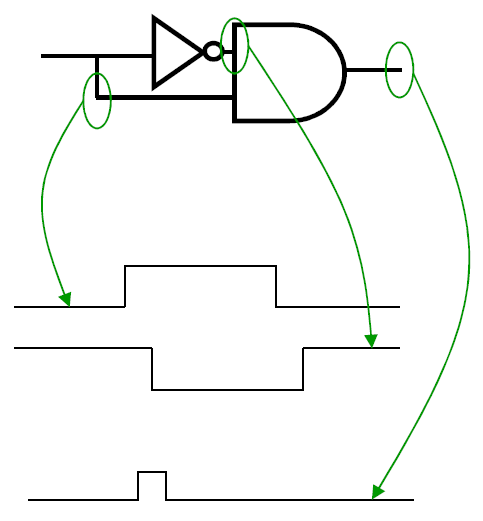
\includegraphics[width = \textwidth]{8_5.png}\caption{Positive Edge Detection}\end{minipage}
\hfill
\begin{minipage}{0.45\textwidth}
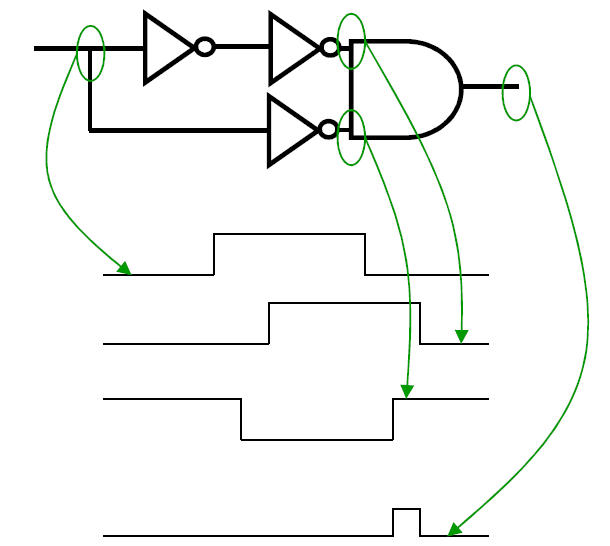
\includegraphics[width = \textwidth]{8_6.png}\caption{Negative Edge Detection}\end{minipage}
\end{figure}
\subsection{$T$ flip-flop}
$T$ flip-flop is the single input version of the $J-K$ flop-flop, formed by $J:=T$ and $K:=T$.\\
When $T=0$, there is no change on $Q$; when $T=1$, $Q$ toggles.
\begin{figure}[h]
\centering
\includegraphics[width = 0.5\textwidth]{8_7.png}
\end{figure}
\clearpage
It admits the following characteristic table:
\begin{table}[h]
\centering
\begin{tabular}{|c|c|c|c|}
\hline
$T$&$CLK$&$Q(t+1)$&\\\hline
0&$\uparrow$&$Q(t)$&No change\\\hline
1&$\uparrow$&$Q(t)^\prime$&Toggle\\\hline
\end{tabular}
\end{table}
From the table, we have $Q(t+1) = T\cdot Q(t)^\prime +T^\prime\cdot Q(t)$.
\subsubsection{Frequency Divider}
Frequency divider can be implemented using a $T$ flip-flop with $T$ set to $1$. Therefore, the output $Q$ will toggle on every rising edge of CLK, effectively making the output half the frequency of the clock.
\begin{figure}[h]
\centering
\includegraphics[width = 0.4\textwidth]{8_8.png}
\end{figure}
\subsubsection{4 bit countdown counter}
The 4 bit countdown counter $ABCD$ which starts from $1111$, can be implemented as follows:
\begin{figure}[h]
\centering
\includegraphics[width = 0.5\textwidth]{8_9.png}
\end{figure}
\subsection{Asynchronous Inputs}
$S-R$, $D$ and $J-K$ inputs are \textbf{synchronous inputs}, as data on these inputs are transferred to the flip-flop's output only on the \textit{triggered} edge of the clock pulse.\\On the other hand, \textbf{asynchronous} inputs affect the state of the flip-flop \textit{indepedent} of the clock. Typical asynchronous inputs are \textbf{preset}(PRE) and \textbf{clear}(CLR).
\begin{itemize}
  \item When PRE = 1, $Q$ is \textit{immediately} set to 1.
  \item When CLR = 1, $Q$ is \textit{immediately} cleared to o.
\end{itemize}
Therefore, flip-flop in normal operation mode when \textit{both} PRE and CLR are low.\\In a sense, PRE and CLR overrides $Q$.\clearpage
\begin{figure}[h]
\centering
\includegraphics[width = 0.6\textwidth]{8_10.png}
\caption{A $J-K$ flop-flop with active low PRESET and CLEAR asynchronous inputs}
\end{figure}
\subsection{Design Methodology for Sequential Logic}
We illustrate the design procedures in the design of 3 bit counter.
\begin{itemize}
  \item[Step 1]Formulate the problem as a truth table.
  \begin{table}[h]
  \centering
  \begin{tabular}{|c|c|c||c|c|c|}
  \hline
  $A(t)$&$B(t)$&$C(t)$&$A(t+1)$&$B(t+1)$&$C(t+1)$\\\hline
  0&0&0&0&0&1\\\hline
  0&0&1&0&1&0\\\hline
  0&1&0&0&1&1\\\hline
  0&1&1&1&0&0\\\hline
  1&0&0&1&0&1\\\hline
  1&0&1&1&1&0\\\hline
  1&1&0&1&1&1\\\hline
  1&1&1&0&0&0\\\hline
  \end{tabular}
  \end{table}
  \item[Step 2]Assign one flip-flop for each of the \textbf{current} state bits $X(t)$.\\Here we use 3 $J-K$ flip-flop for $A$, $B$, $C$.
  \item[Step 3]Draw truth table for flip-flop inputs. Note any output will be dependent on \textbf{all} the input.\clearpage
  \begin{table}[h]
  \centering
  \begin{tabular}{|c|c|c||c|c|c|c|c|}
  \hline
  $A(t)$&$B(t)$&$C(t)$&$A(t+1)$&$B(t+1)$&$C(t+1)$&$J_A$&$K_A$\\\hline
  0&0&0&0&0&1&0&X\\\hline
  0&0&1&0&1&0&0&X\\\hline
  0&1&0&0&1&1&0&X\\\hline
  0&1&1&1&0&0&1&X\\\hline
  1&0&0&1&0&1&X&0\\\hline
  1&0&1&1&1&0&X&0\\\hline
  1&1&0&1&1&1&X&0\\\hline
  1&1&1&0&0&0&X&1\\\hline
  \end{tabular}
  \end{table}
    \item[Step 4] Using K map, generate minimum SOP for all inputs in the assigned flip-flops.\\
  \begin{align*}
  J_A&=BC\\
  K_A&=BC
  \end{align*}
  \item[Step 5] Implement in circuit
  \begin{figure}[h]
  \centering
  \includegraphics[width = 0.7\textwidth]{8_11.png}
  \end{figure}
\end{itemize}
\subsection{Metastability}
In reality, nothing is instantaneous. Data will have a \textbf{setup time} $t_s$ and a \textbf{hold time} $t_h$ to observe, while \textbf{clock-to-ouput time} $t_\text{co}$, which is the propagation delay, is associated with the clock and output.\clearpage
\begin{figure}[h]
\centering
\includegraphics[width = 0.5\textwidth]{8_12.png}
\end{figure}
\textbf{Metastability} is introduced if setup and hold times are violated, as flip-flop may oscillate in an indeterminate state between 0 and 1.
Although metastability cannot be absolutely avoided in practice, two way to resolve it can be
\begin{itemize}
  \item Make sure clock period is long enough.
  \item Use flip-flop chain
  \begin{figure}[h]
  \centering
  \includegraphics[width = 0.5\textwidth]{8_13.png}
  \end{figure}
  Probability of metastability gets closer and closer to zero as number of flip-flops connected in series increase.
\end{itemize}
\subsection{Memory Hierarchy}
\textbf{Memory} stores programs and data.\\
\begin{figure}[h]
\begin{minipage}{0.4\textwidth}
We define
\begin{itemize}
  \item 1 byte = 8 bits
  \item 1 KB = $2^{10}$ bytes
  \item 1 MB = $2^{20}$ bytes
  \item 1 GB = $2^{30}$ bytes
  \item 1 TB = $2^{40}$ bytes
\end{itemize}
\end{minipage}\hfill
\begin{minipage}{0.5\textwidth}
\centering
\includegraphics[width = \textwidth]{8_14.png}
\end{minipage}\end{figure}
\clearpage
\section{Understanding Performance}
\subsection{Defining Performance}
To improve performance, we are interested to minimise
\begin{itemize}
  \item Response time/\textbf{Execution time}: the time between the start and the completion of a task.\\
  Execution time is \textit{inversely} related to the performance.
  \[
\text{performance} = \frac{1}{\text{execution time}}
  \] 
  \item \textbf{Throughput} -- Total amount of work done in a given time\\
  Decreasing response time always improves throughput.
\end{itemize}
\textbf{Remark:} \textit{elapsed} time do not equal execution time.
\begin{itemize}
  \item CPU execution time(CPU time) is the time CPU spends working on a task
  \item CPU execution time does \textit{not} include time (1) waiting for I/O or (2) running other programmes.
\end{itemize}
\subsection{CPU Execution Time}
\begin{definition}[CPU Execution Time]
\hfill\\\normalfont CPU execution time for a program is given by
\begin{align*}
\text{CPU execution time} &= {\# \text{ of CPU clock cycle}}\times\text{clock cycle time (s)}\\
&=\frac{\#\text{ of CPU clock cycle}}{\text{clock rate (Hz)}}
\end{align*}
\end{definition}
Therefore, there are 2 ways to improve performance, by either
\begin{enumerate}
  \item Reducing the length of the clock cycle, or
  \item Reducing the \# of clock cycles required for a program
\end{enumerate}
\begin{definition}[Clock Rate]
\hfill\\\normalfont Clock rate is the inverse of clock cycle time.
\[
\text{Clock rate(CR)} = \frac{1}{\text{Clock Cycle Time(CC)}}
\]
\begin{figure}[h]
\centering
\includegraphics[width = 0.6\textwidth]{9_1.png}
\end{figure}
\end{definition}
\subsection{Clock Cycles per Instruction}
Different instructions take different amount of time to execute. On average, we have
\[
\text{\# of CPU cycles} = \text{\# of Instructions}\times\text{Average Clock Cycles per Instruction(CPI)}
\]
where Clock Cycles per Instruction is defined as:
\begin{definition}[Clock Cycle per Instruction]
\hfill\\\normalfont \textbf{Clock cycles per instruction} is the average number of clock cycles each instruction takes to execute.
\end{definition}
This allows the measurement of clock cycles per instruction for different instruction class. \\Overall, we can calculate \textbf{effective CPI} defined as below.
\begin{definition}[Effective CPI]
\hfill\\\normalfont Overall effective CPI is calculated by a weighted average of clock cycle per instruction among all classes of instructions.
\[
\text{Overall effective CPI} = \sum_{i\in I} \text{CPI}_i\times\text{IC}_i
\]
where IC stands for the \textbf{percentage} of instruction count, serving as the weight.
\end{definition}
\subsection{CPU performance}
\begin{definition}[Performance Equation]
\hfill\\\normalfont The performance equation of CPU is
\[
\text{CPU time} = \text{instruction count(IC)}\times\text{CPI}\times\text{clock cycle} = \frac{\text{IC}\times\text{CPI}}{\text{clock rate}}
\]
\end{definition}
This equation gives us a way to calculate average CPI.

There are multiple factors affecting CPU performance.
\begin{table}[h]
\centering
\begin{tabular}{|l|c|c|c|}
\hline
&Instruction Count&CPI&Clock Cycle\\\hline
Algorithm&*&*&\\\hline
Programming language&*&*&\\\hline
Compiler&*&*&\\\hline
ISA&*&*&*\\\hline
Processor Organisation&&*&*\\\hline
Technology&&&*\\\hline
\end{tabular}
\end{table}
\clearpage
\end{document}